\documentclass[a4paper,10pt]{article}

\usepackage{tabularx} % extra features for tabular environment
\usepackage{amsmath}  % improve math presentation
\usepackage{graphicx} % takes care of graphic including machinery
\usepackage[margin=1in,letterpaper]{geometry} % decreases margins
\usepackage{cite} % takes care of citations
\usepackage[final]{hyperref} % adds hyper links inside the generated pdf file
\usepackage{ctex}
\usepackage{titlesec}
%\usepackage{CJKutf8, CJK}
\usepackage{makecell}                 % 三线表-竖线
\usepackage{booktabs}                 % 三线表-短细横线
% \usepackage{natbib}
\usepackage{graphicx}				  % 表格单元格逆时针
\usepackage{multirow}				  % 合并单元格
\usepackage{array}
\usepackage{amssymb}				  % 勾
\usepackage{amsmath}
\usepackage{longtable}                % 导入 longtable 宏包,表格自动换行
\usepackage{caption}
\usepackage{subcaption}               % 设置子图
\usepackage{color}					  % 文本颜色包
\usepackage{xcolor}
\usepackage{bbm}					  % 输入指示函数
\usepackage{tablefootnote}			  % 表格注释
\usepackage{pythonhighlight}
\usepackage{fancyhdr}
\usepackage{lastpage}
\pagestyle{fancy}
\fancyhf{}
\fancyhead{}
\fancyfoot{}
\fancyhead[R]{\small Page \thepage\ of \pageref*{LastPage}}
\fancyhead[L]{\small Report}

\usepackage{listings}                 % 导入代码块
\usepackage{xcolor}
\lstset{
	numbers=left, 
	tabsize=1,
	columns=flexible, 
	numberstyle=  \small, 
	keywordstyle= \color{ blue!70},
	commentstyle= \color{red!50!green!50!blue!50}, 
	frame=shadowbox, % 阴影效果
	rulesepcolor= \color{ red!20!green!20!blue!20} ,
	escapeinside=``, % 英文分号中可写入中文
	xleftmargin=2em,
	xrightmargin=2em, 
	aboveskip=1em,
} 

\hypersetup{
	colorlinks=true,       % false: boxed links; true: colored links
	linkcolor=blue,        % color of internal links
	citecolor=blue,        % color of links to bibliography
	filecolor=magenta,     % color of file links
	urlcolor=blue         
}
%++++++++++++++++++++++++++++++++++++++++
\titleformat{\section}{\Large\bfseries\songti}{\thesection}{1em}{}
\titleformat{\subsection}{\large\bfseries\songti}{\thesubsection}{1em}{}
\titleformat{\subsubsection}{\normalsize\bfseries\songti}{\thesubsubsection}{1em}{}
\titleformat{\paragraph}{\small\bfseries\songti}{\paragraph}{1em}{}
\titleformat{\subparagraph}{\footnotesize\bfseries\songti}{\subparagraph}{1em}{}

\begin{document}
	
	
	\title{\songti \zihao{4}Unity VR 项目开发进度}
%	\author{\textrm{Ku Jui}}
	\date{\textrm{September 2023}}
	\maketitle
	
	\renewcommand{\figurename}{Figure} % 可以重新定义abstract,因为ctex会覆盖thebibliography
	% 	\begin{abstract}
		%		In this experiment we studied a very important physical effect by measuring the
		%		dependence of a quantity $V$ of the quantity $X$ for two different sample
		%		temperatures.  Our experimental measurements confirmed the quadratic dependence
		%		$V = kX^2$ predicted by Someone's first law. The value of the mystery parameter
		%		$k = 15.4\pm 0.5$~s was extracted from the fit. This value is
		%		not consistent with the theoretically predicted $k_{theory}=17.34$~s. We attribute %this
		%		discrepancy to low efficiency of our $V$-detector.
		%	\end{abstract}
	\renewcommand{\contentsname}{Contents}
	\renewcommand{\tablename}{Table}
	\tableofcontents  % 自动生成目录
	
	\section{项目需求}
		
		\subsection{船只模型自定义}
		
		\begin{figure}[htbp]
			% read manual to see what [ht] means and for other possible options
			\centering				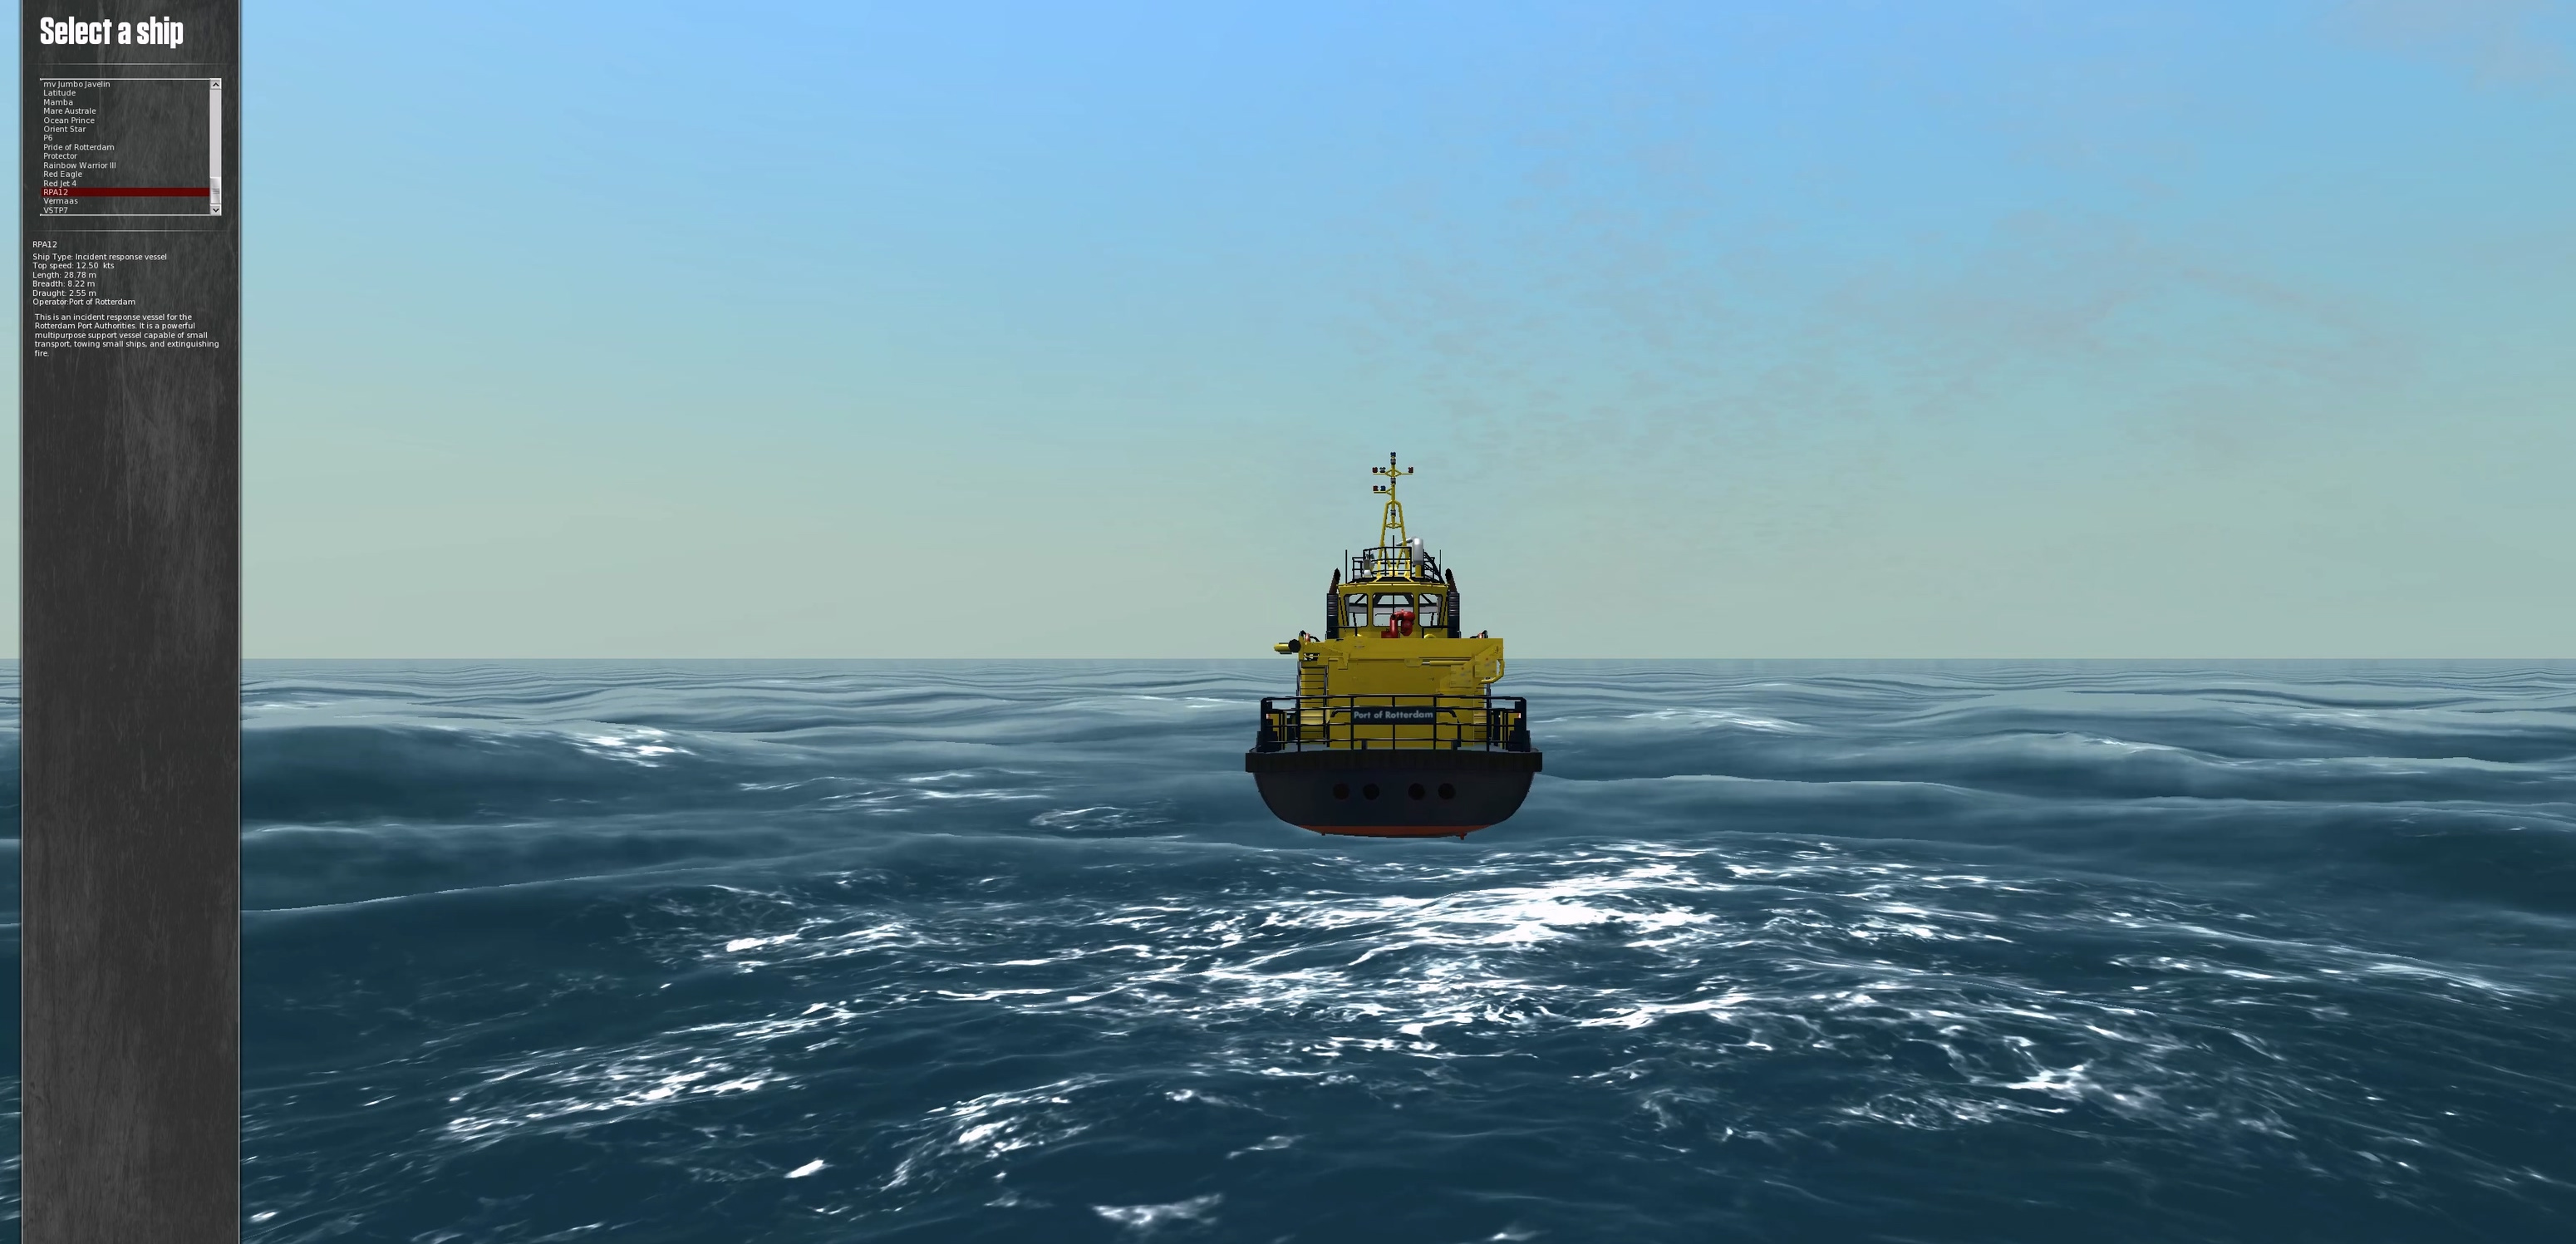
\includegraphics[width=\columnwidth]{picture/Select a ship}
			%\captionsetup{font=scriptsize}
			\caption{
				\label{fig: Select a ship} 
				船只模型选择界面示意图。
			}	
		\end{figure}
		
		玩家可以进行船只选择,不同的船只会有区别,如转向半径、平稳程度、马力、船只大小等会有明显区别。并且进行选择时,该船只会出现在主界面上,玩家可以直观的看到所选择的船只模型,如 Fig. \ref{fig: Select a ship}所示,且\textbf{至少有两个船只类别}。
		
		\subsection{天气系统功能实现}
		
		前期开发需要\textbf{实现两种海面天气,如 Hail 和 Storm 天气},如 Fig. \ref{fig: Hail}和 Fig. \ref{fig: Storm}所示。
		
		\begin{figure}[htbp] 
			% read manual to see what [ht] means and for other possible options
			\centering 
			% 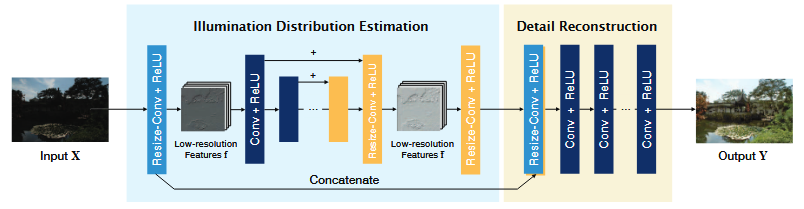
\includegraphics[width=0.8\columnwidth]{GLADNet}
			
			\begin{subfigure}{0.3\textwidth}
				\includegraphics[width=\linewidth]{picture/Clear sky}
				\captionsetup{font=scriptsize}
				\caption{Clear sky}
				\label{fig: Clear sky}
			\end{subfigure}
			\begin{subfigure}{0.3\textwidth}
				\includegraphics[width=\linewidth]{picture/Drizzle}
				\captionsetup{font=scriptsize}
				\caption{Drizzle}
				\label{fig: Drizzle}
			\end{subfigure}
			\begin{subfigure}{0.3\textwidth}
				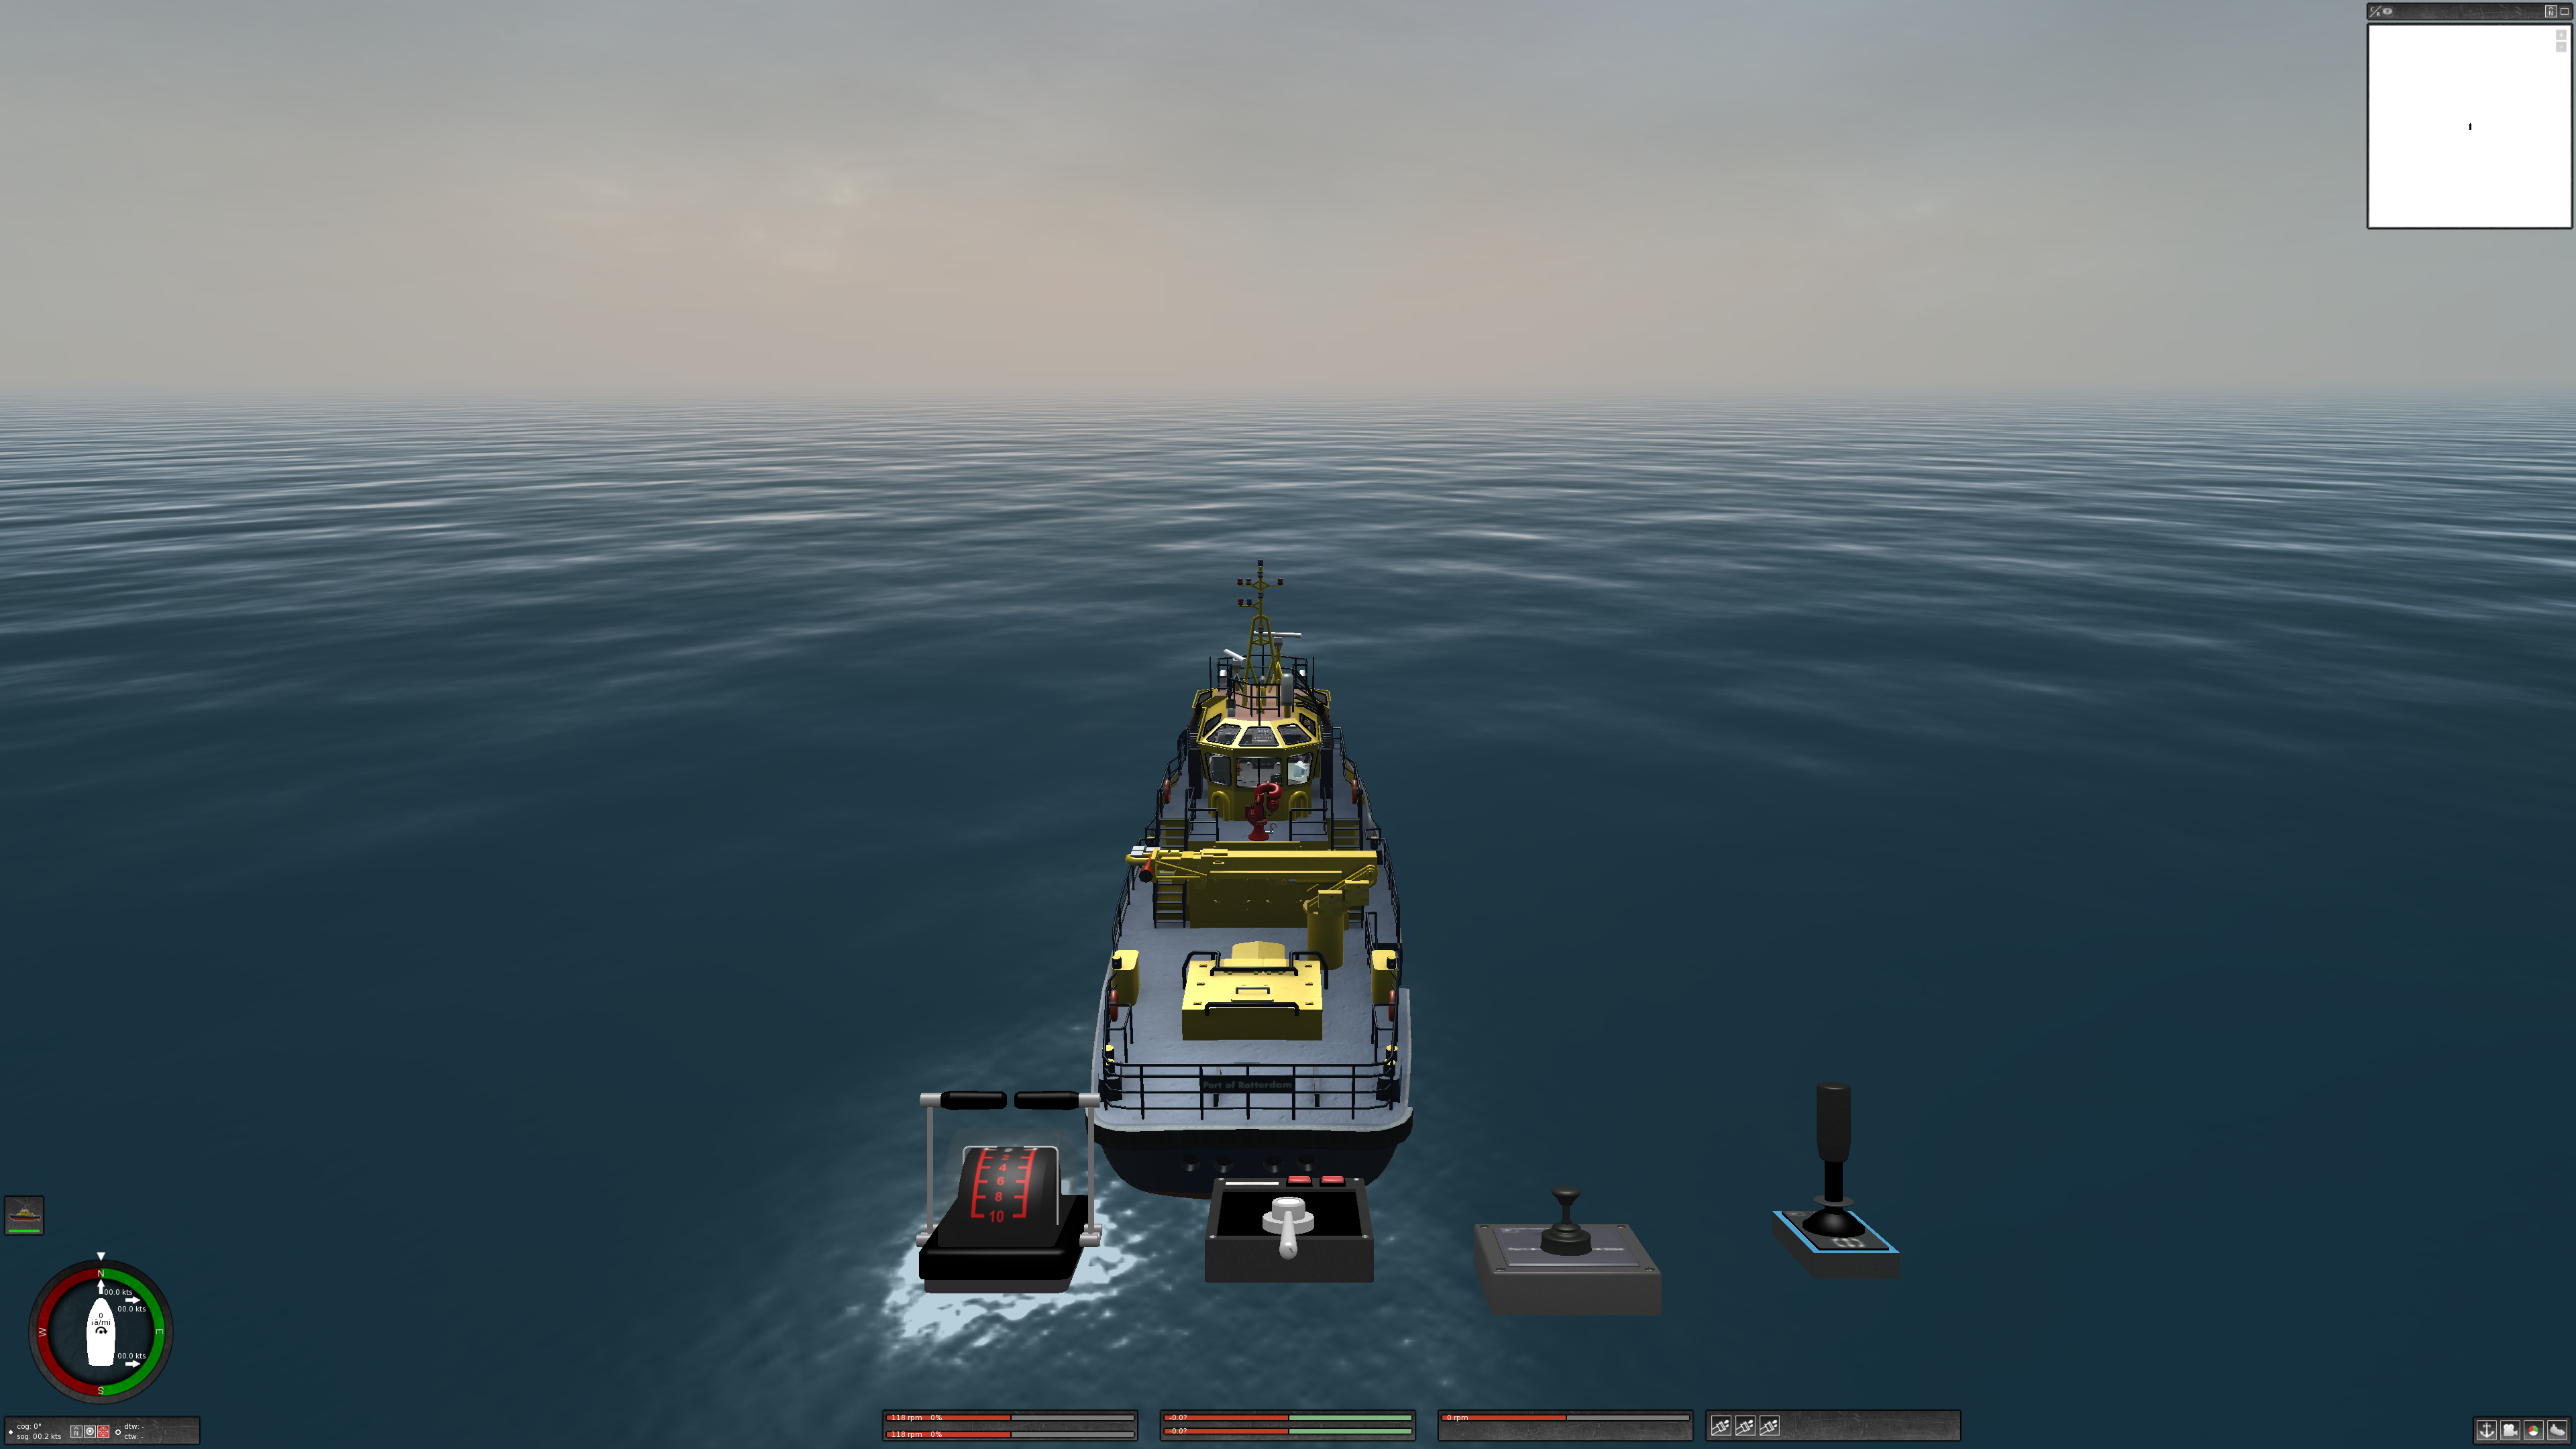
\includegraphics[width=\linewidth]{picture/Foggy}
				\captionsetup{font=scriptsize}
				\caption{Foggy}
				\label{fig: Foggy}	
			\end{subfigure}\\
			\begin{subfigure}{0.3\textwidth}
				\includegraphics[width=\linewidth]{picture/Hail}
				\captionsetup{font=scriptsize}
				\caption{Hail}
				\label{fig: Hail}	
			\end{subfigure}
			\begin{subfigure}{0.3\textwidth}
				\includegraphics[width=\linewidth]{picture/Light snow}
				\captionsetup{font=scriptsize}
				\caption{Light snow}
				\label{fig: Light snow}
			\end{subfigure}
			\begin{subfigure}{0.3\textwidth}
				\includegraphics[width=\linewidth]{picture/Rainy}
				\captionsetup{font=scriptsize}
				\caption{Rainy}
				\label{fig: Rainy}
			\end{subfigure}\\
			\begin{subfigure}{0.3\textwidth}
				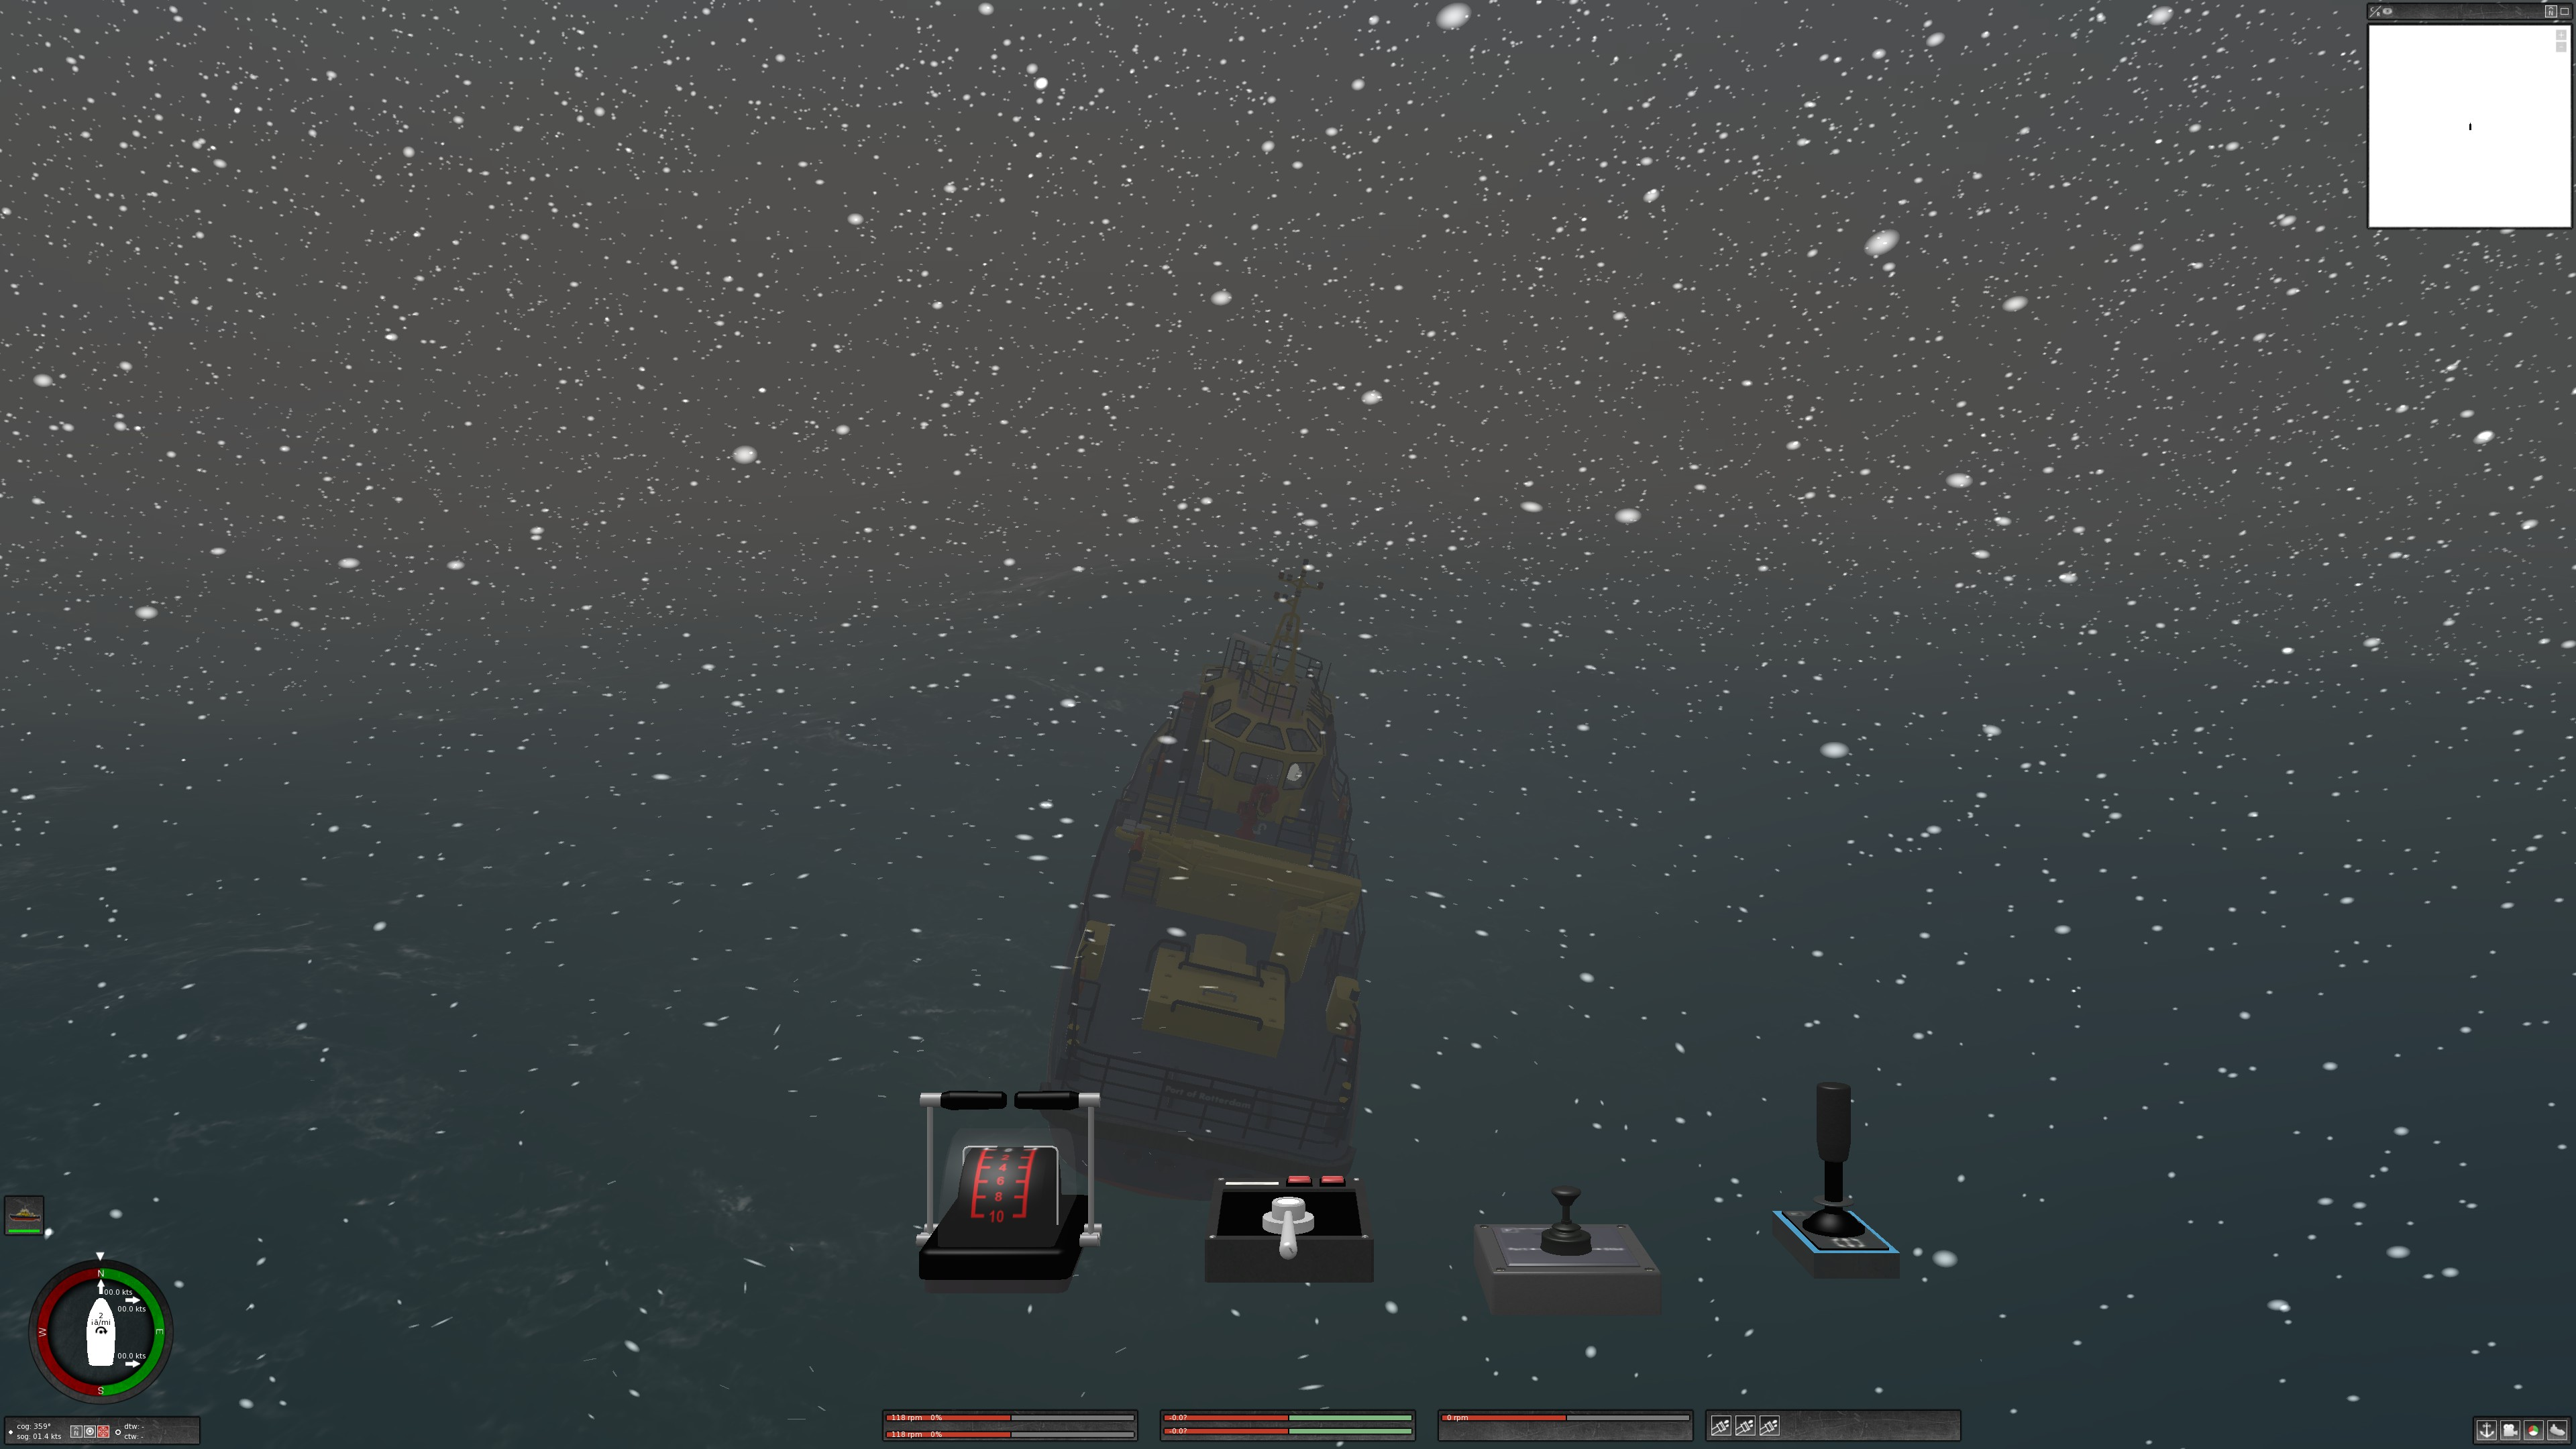
\includegraphics[width=\linewidth]{picture/Snow storm}
				\captionsetup{font=scriptsize}
				\caption{Snow storm}
				\label{fig: Snow storm}	
			\end{subfigure}
			\begin{subfigure}{0.3\textwidth}
				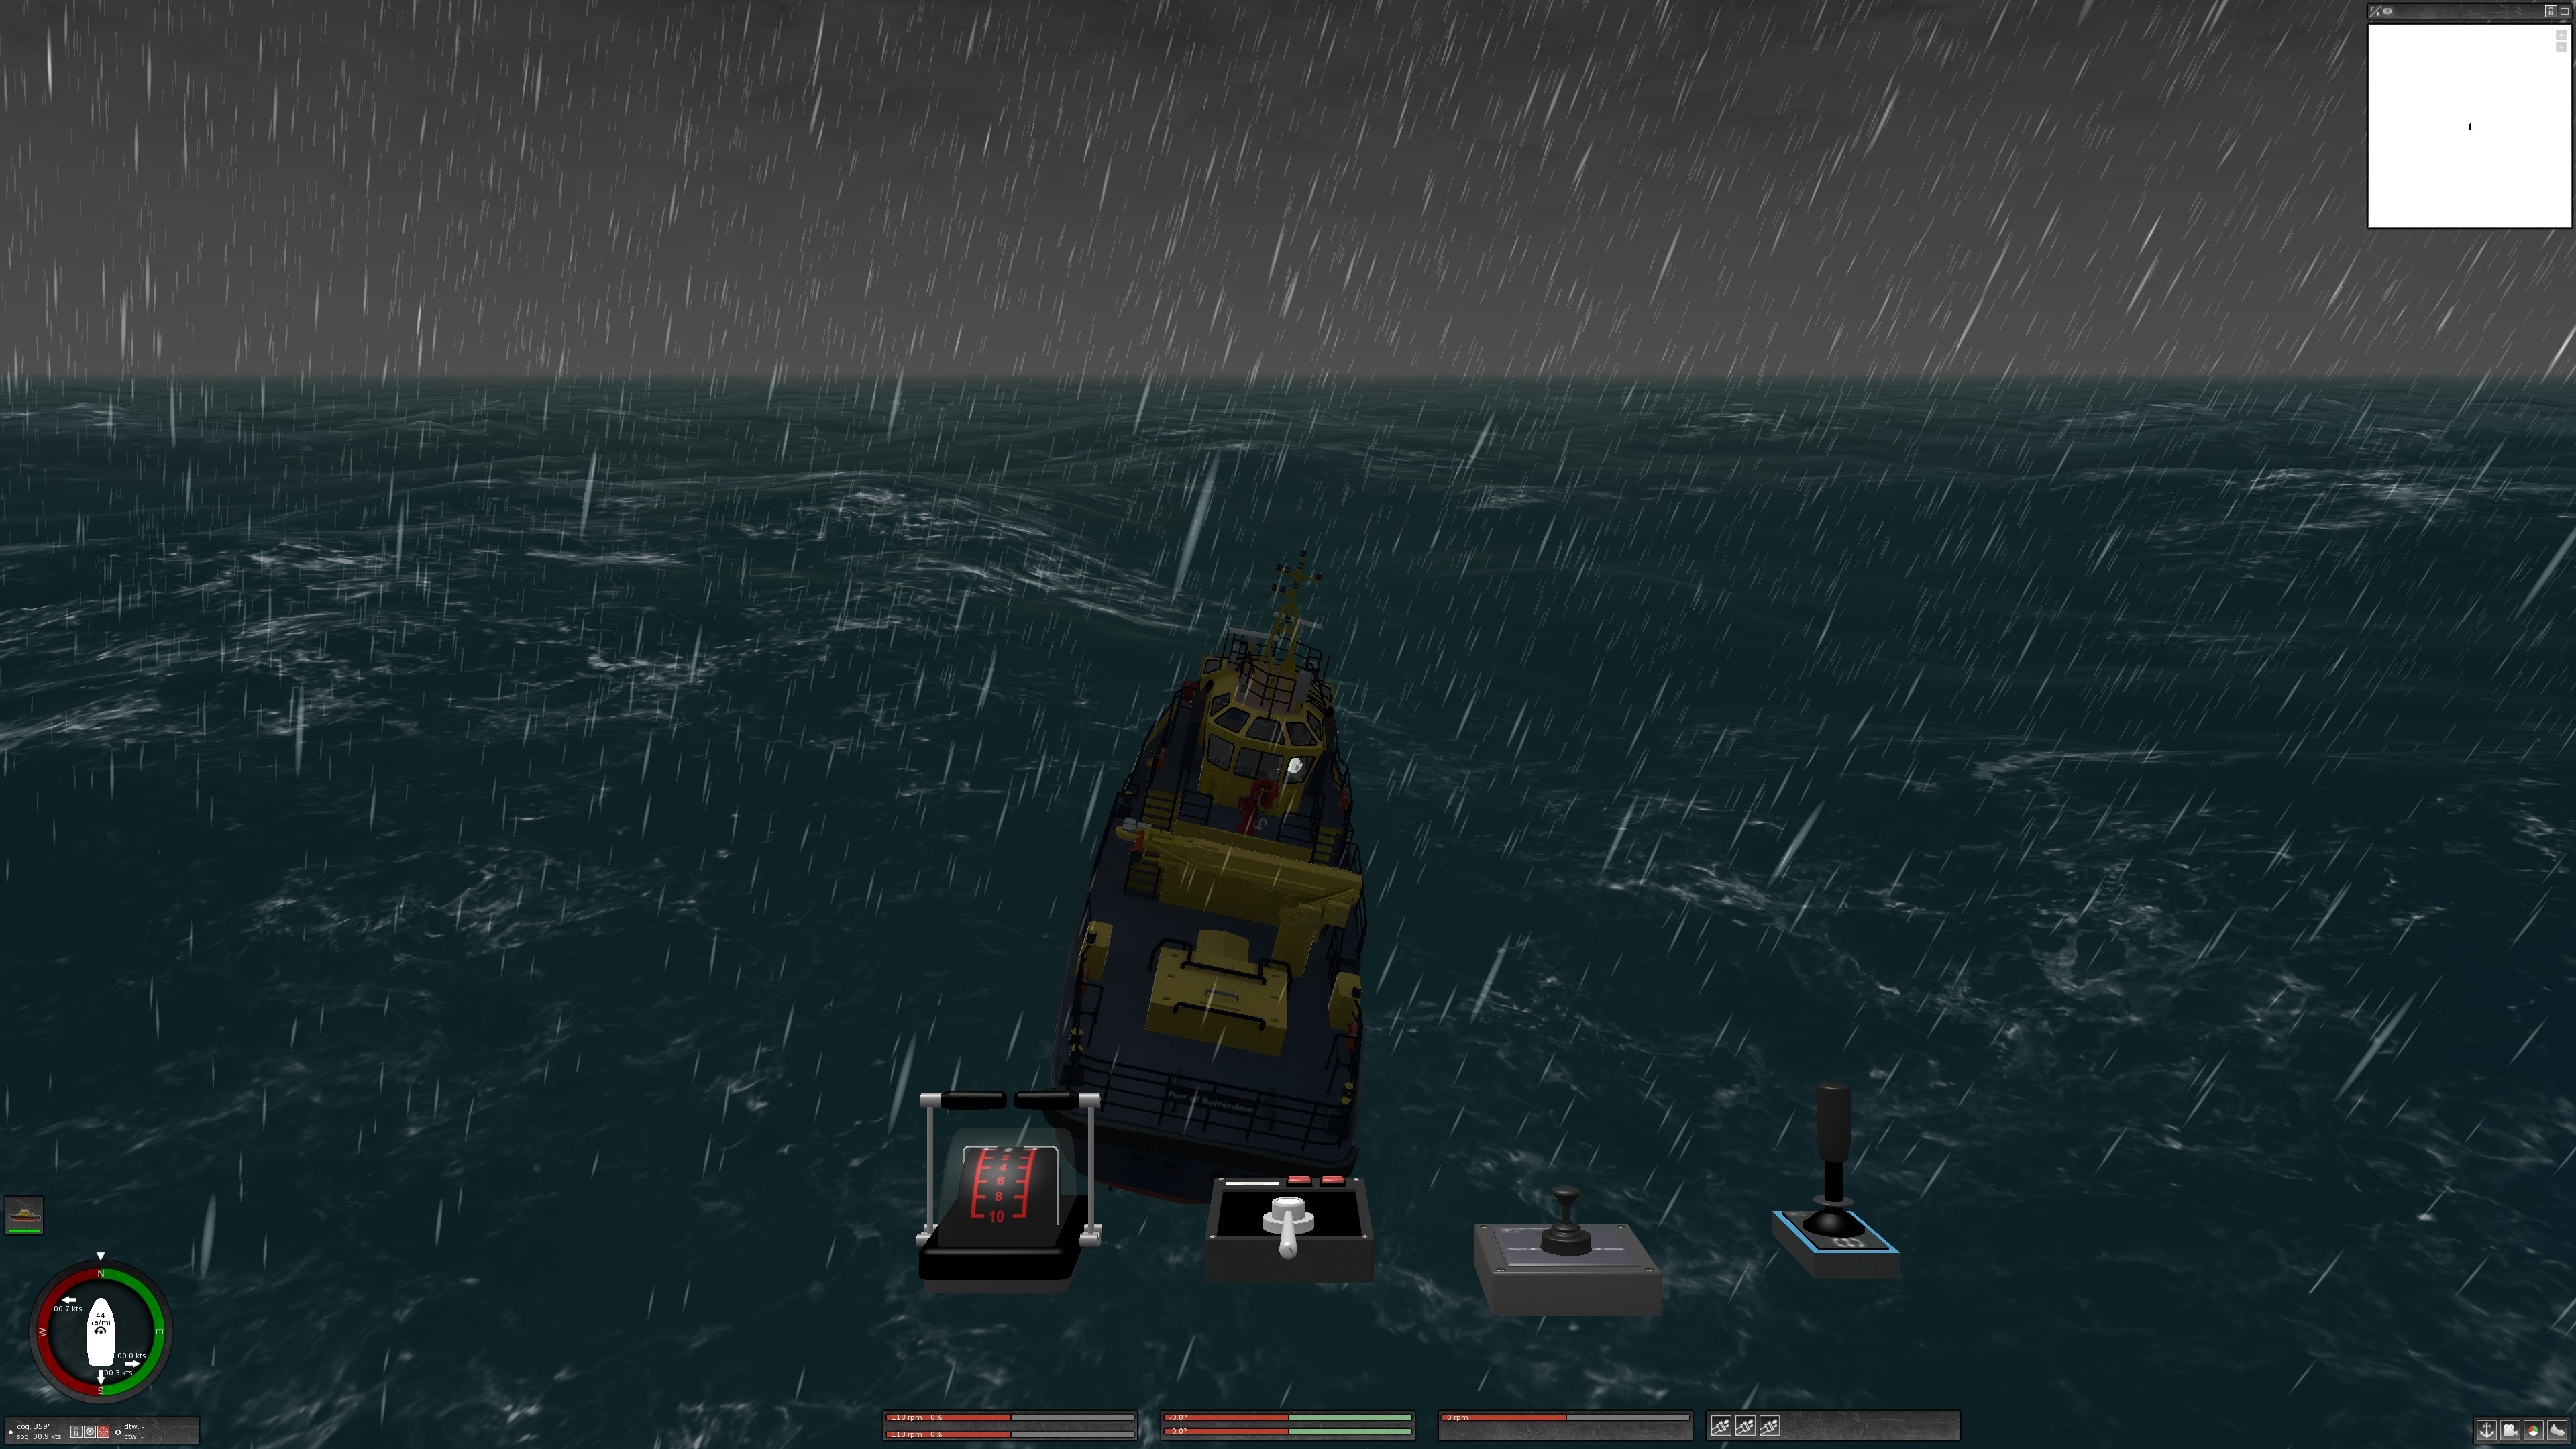
\includegraphics[width=\linewidth]{picture/Storm}
				\captionsetup{font=scriptsize}
				\caption{Storm}
				\label{fig: Storm}	
			\end{subfigure}
			\begin{subfigure}{0.3\textwidth}
				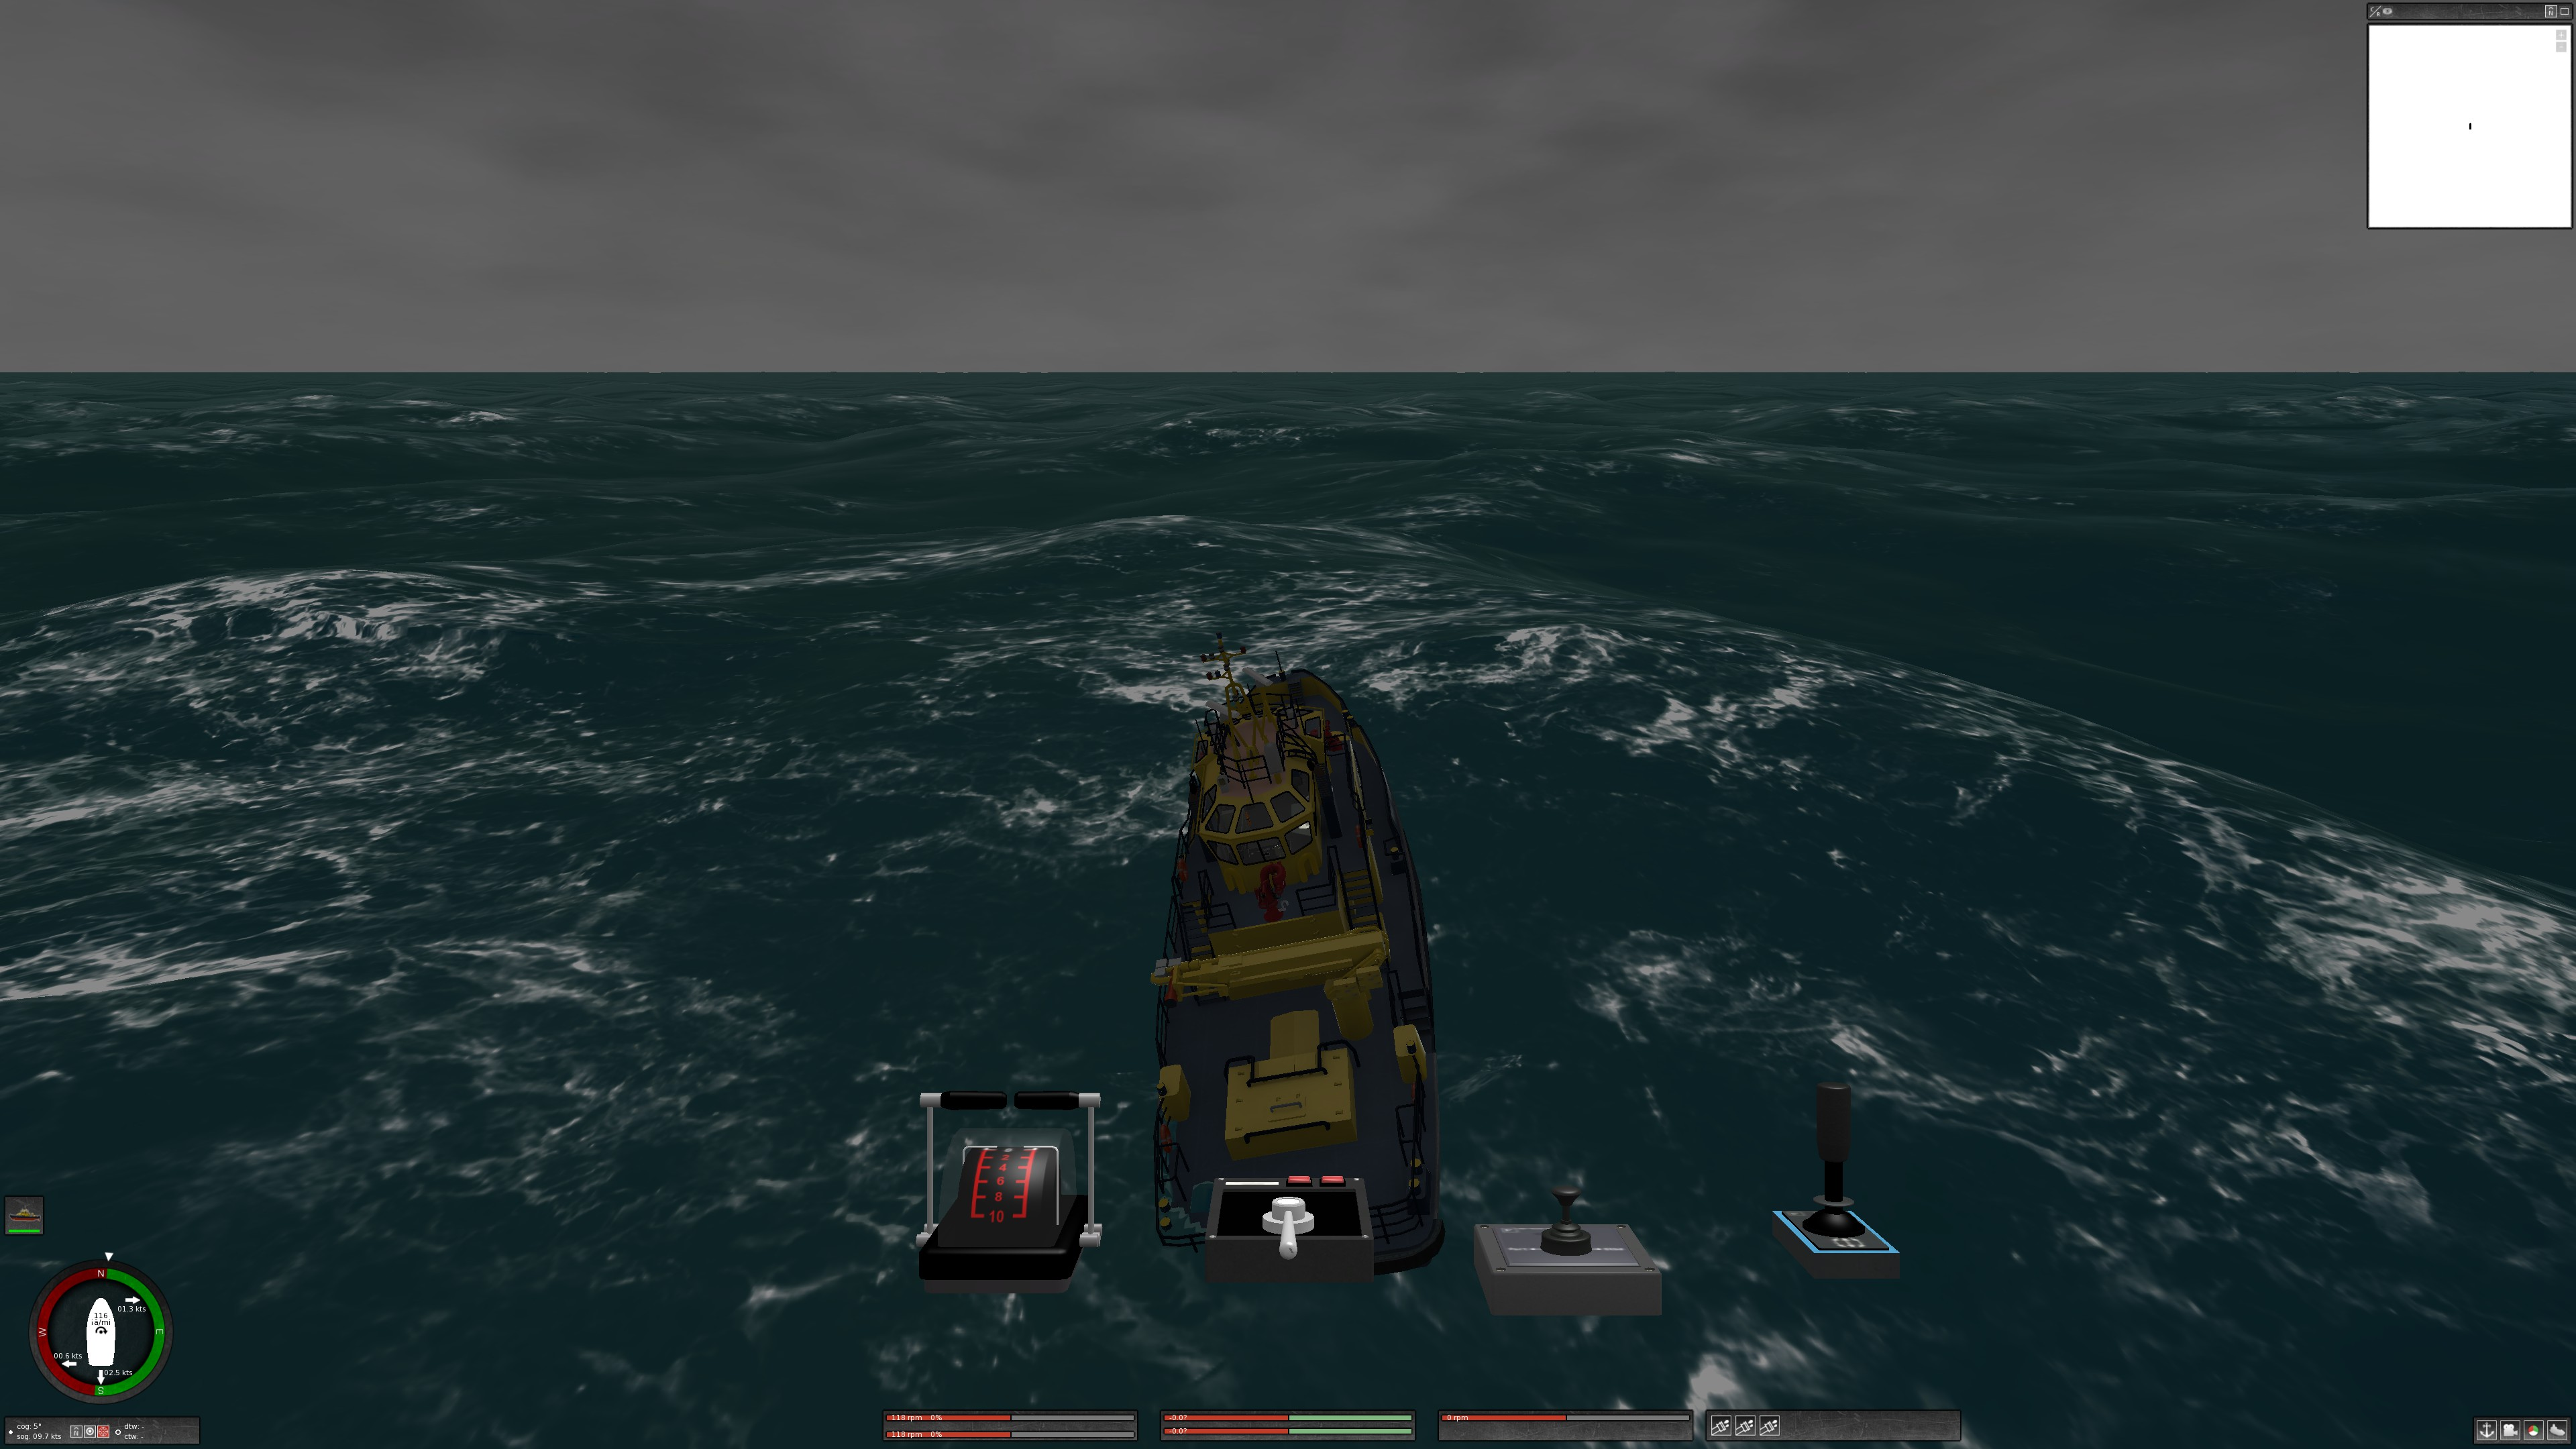
\includegraphics[width=\linewidth]{picture/Wind}
				\captionsetup{font=scriptsize}
				\caption{Wind}
				\label{fig: Wind}
			\end{subfigure}
			\captionsetup{font=scriptsize}
			\caption{
				\label{fig: Weather}
				9种不同的天气下的海况表现
			}
		\end{figure}
		
		其中 \textbf{Storm} 海况下(强风、大浪、降水),海面需要实现\textbf{明显且逼真}的波涛汹涌效果,船只随着海浪的涌动而剧烈摇晃,天空阴云密布,下暴雨;在 \textbf{Hail} 海况下,海面白色浪花更加明显,海水波动效果明显,能见度低,远处阴云密布,下冰雹。
		
		\subsection{操作视角自定义}
		
		玩家在操纵船只时,可以选择不同的操作视角,主要有两种游戏视角,分别为 orbit(航线视角), helmsman(舵手视角), 如Fig. \ref{fig: View}所示。
		
		\begin{figure}[htbp] 
			% read manual to see what [ht] means and for other possible options
			\centering 
			% 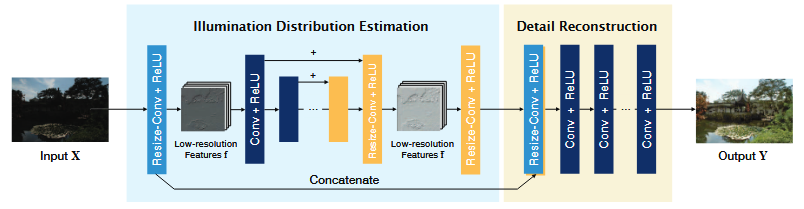
\includegraphics[width=0.8\columnwidth]{GLADNet}
			
			\begin{subfigure}{0.3\textwidth}
				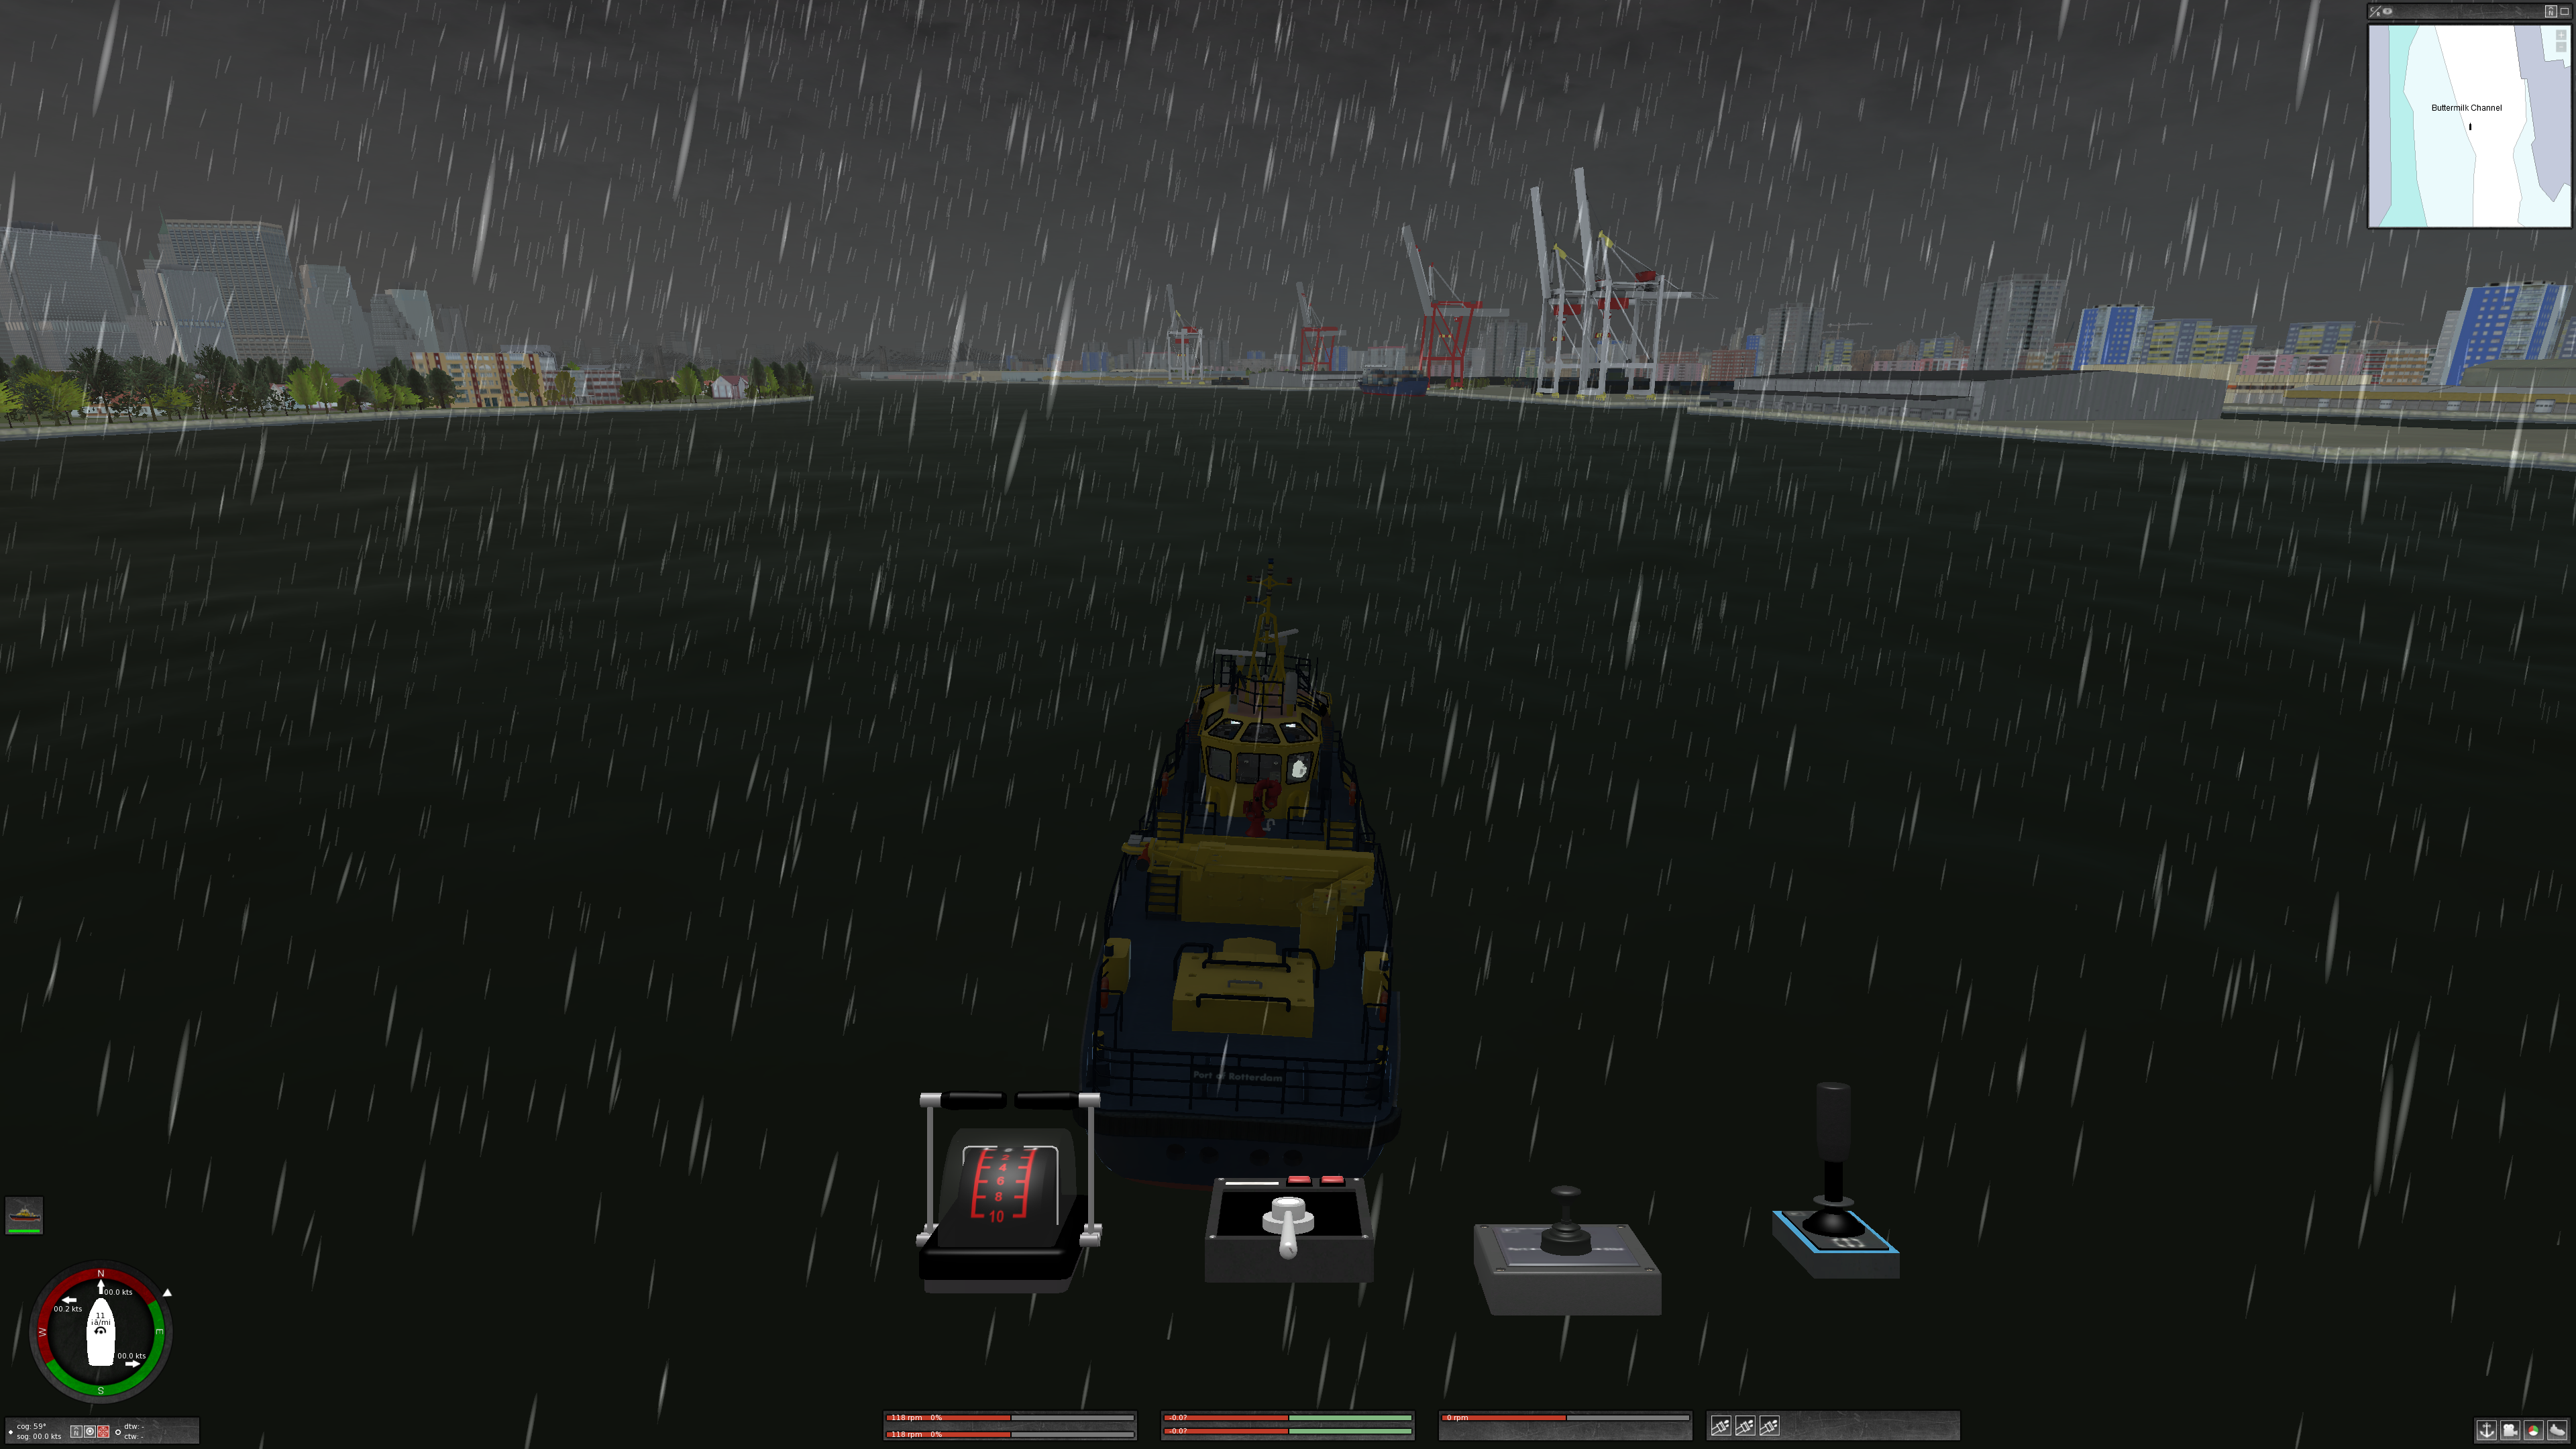
\includegraphics[width=\linewidth]{picture/orbit}
				\captionsetup{font=scriptsize}
				\caption{orbit}
				\label{fig: orbit}
			\end{subfigure}
			\begin{subfigure}{0.3\textwidth}
				\includegraphics[width=\linewidth]{picture/helmsman}
				\captionsetup{font=scriptsize}
				\caption{helsman}
				\label{fig: helmsman}
			\end{subfigure}
			\captionsetup{font=scriptsize}
			\caption{
				\label{fig: View}						
				2种不同的操控视角。
			}
		\end{figure}
		
		\begin{figure}[htbp]
			% read manual to see what [ht] means and for other possible options
			\centering				\includegraphics[width=\columnwidth]{picture/Hail}
			%\captionsetup{font=scriptsize}
			\caption{
				\label{fig: Hail1} 
				Hail海况
			}	
		\end{figure}
		
		\begin{figure}[htbp]
			% read manual to see what [ht] means and for other possible options
			\centering				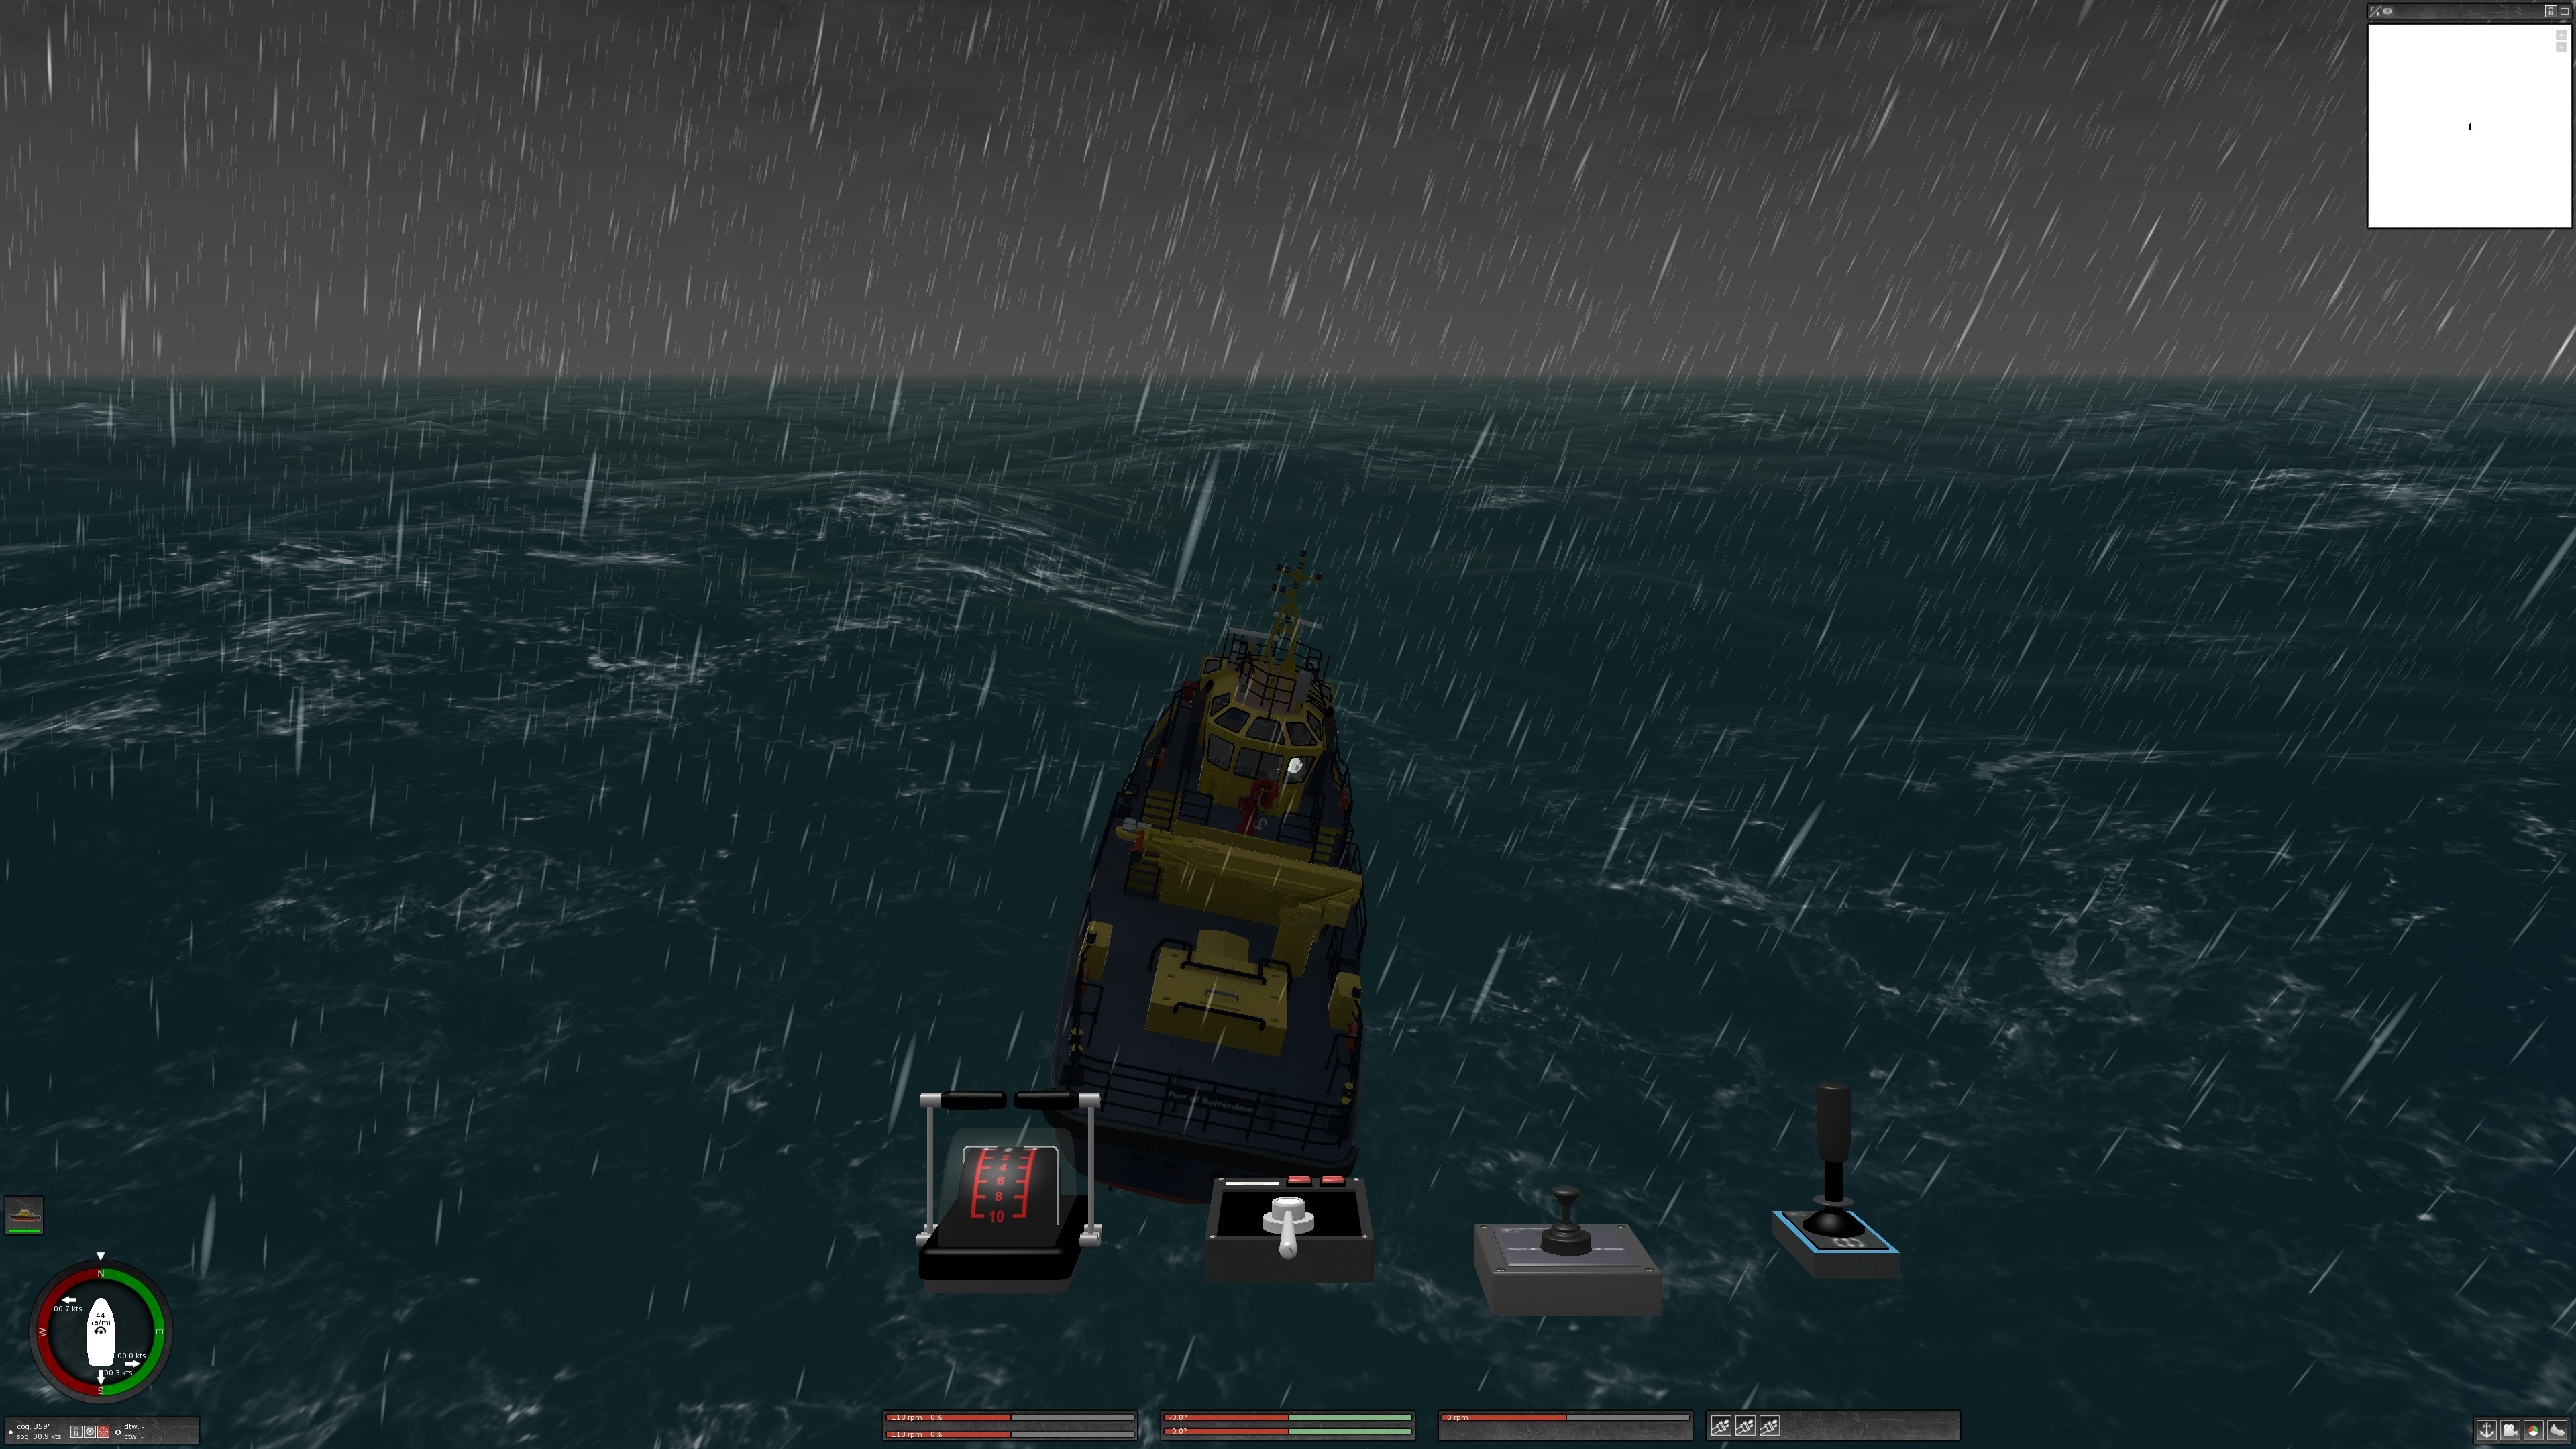
\includegraphics[width=\columnwidth]{picture/Storm}
			%\captionsetup{font=scriptsize}
			\caption{
				\label{fig: Storm1} 
				Storm海况
			}	
		\end{figure}
		
		\subsection{VR沉浸式体验装置}
		
		一种虚拟现实单人体感平台体验装置,包括底板、气缸和基座,安全座地段体感仓的外侧均匀通过铰接件安装有三自由度电动缸,电动缸由控制器控制。该装置能够模拟船只海面航行的状态,根据模拟船只的航行状态,通过气缸的左右推动模拟出海面船只颠簸效果。
		
		为了实现VR游戏中海面海浪波动参数的传递到装置控制器或提供相关接口以便后续开发,有以下需求:
		
		
		\begin{itemize}
			\item[(1)] 
			\textbf{设备控制器反馈}:确保游戏支持VR控制器的反馈功能,这可以通过适当的API和SDK来实现。具体来说,你可以使用控制器的震动反馈来传达海浪波动的强度和频率给玩家。这需要游戏引擎和VR平台的支持。
			
			\item[(2)]
			外部控制接口:为了方便后续开发,可以设计一个接口或者提供API,允许开发人员访问游戏中海浪波动的参数。这个接口可以提供有关海浪高度、波浪频率、风力等信息,并允许其他应用程序或设备根据这些参数进行调整。
			
			\item[(3)]
			数据输出:游戏可以将海浪波动参数以实时数据流或事件的形式输出到外部系统。这允许其他开发者编写自定义控制器或设备,以根据海浪情况来调整虚拟船只的运动。
			
			\item[(4)]
			开发者文档:提供详细的开发者文档,解释了如何使用游戏中的接口或API来获取海浪波动参数。这有助于其他开发者更容易地集成游戏的功能。
			
		\end{itemize}	
		
	\section{开发进度}
	
		开发项目演示视频见\footnote{https://github.com/npukujui11/npukujui11/tree/Unity-VR/LaTeX/assignment/Unity-VR/Progress-report/video}
	
		\subsection{场景开发进度}
		
		目前已经开发了三种不同的天气场景,分别是雾天 (Foggy) 、下雨天 (Rainy)和冰雹天气 (Hail),见 Fig .\ref{fig: Third-person perspective another-IP}, Fig .\ref{fig: Third-person perspective another rain-IP}, Fig .\ref{fig: Third-person perspective another hail-IP}。
		
		\begin{figure}[htbp] 
			% read manual to see what [ht] means and for other possible options
			\centering 
			% 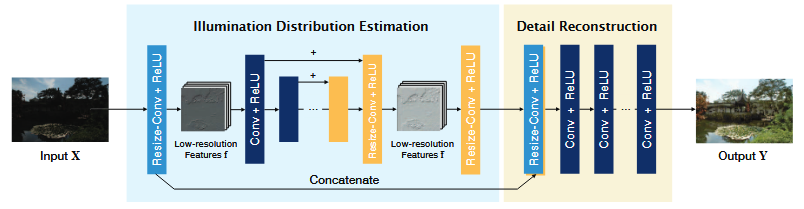
\includegraphics[width=0.8\columnwidth]{GLADNet}
			
			\begin{subfigure}{0.3\textwidth}
				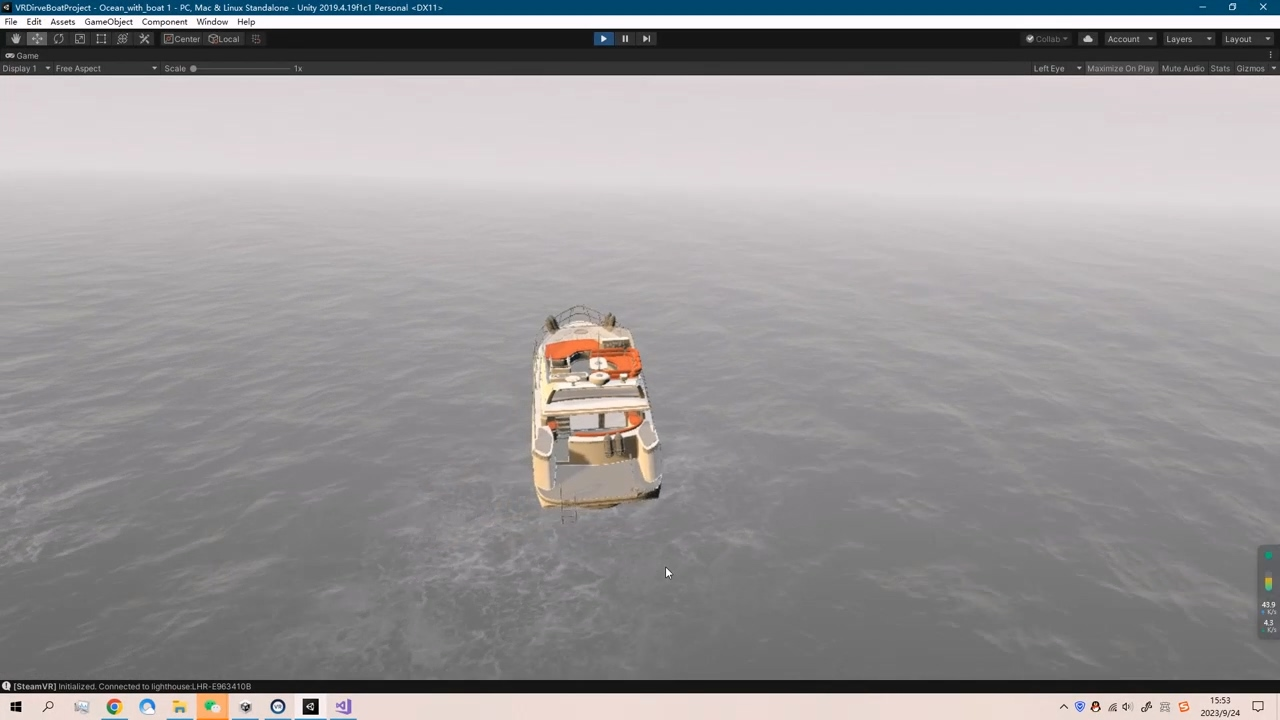
\includegraphics[width=\linewidth]{picture/Third-person perspective another-IP}
				\captionsetup{font=scriptsize}
				\caption{Foggy}
				\label{fig: Third-person perspective another-IP}
			\end{subfigure}
			\begin{subfigure}{0.3\textwidth}
				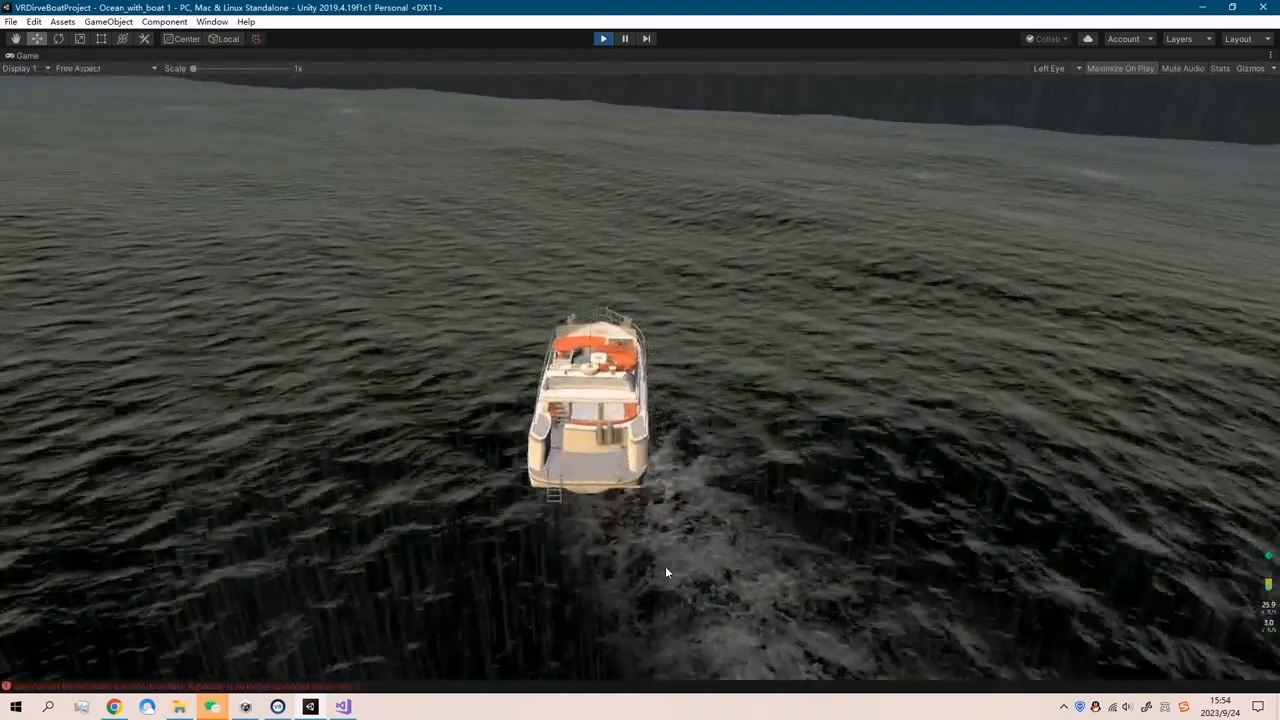
\includegraphics[width=\linewidth]{picture/Third-person perspective another rain-IP}
				\captionsetup{font=scriptsize}
				\caption{Rainy}
				\label{fig: Third-person perspective another rain-IP}
			\end{subfigure}
			\begin{subfigure}{0.3\textwidth}
				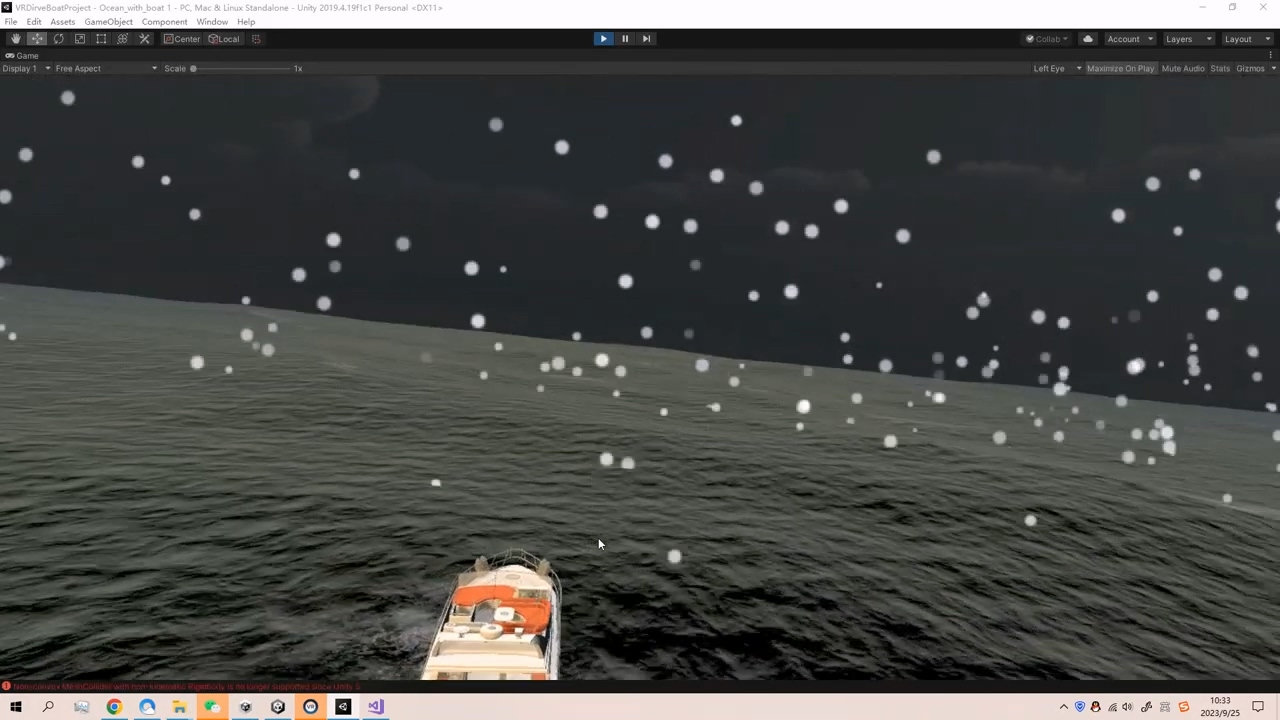
\includegraphics[width=\linewidth]{picture/Third-person perspective another hail-IP}
				\captionsetup{font=scriptsize}
				\caption{Hail}
				\label{fig: Third-person perspective another hail-IP}	
			\end{subfigure}\\
			\begin{subfigure}{0.3\textwidth}
				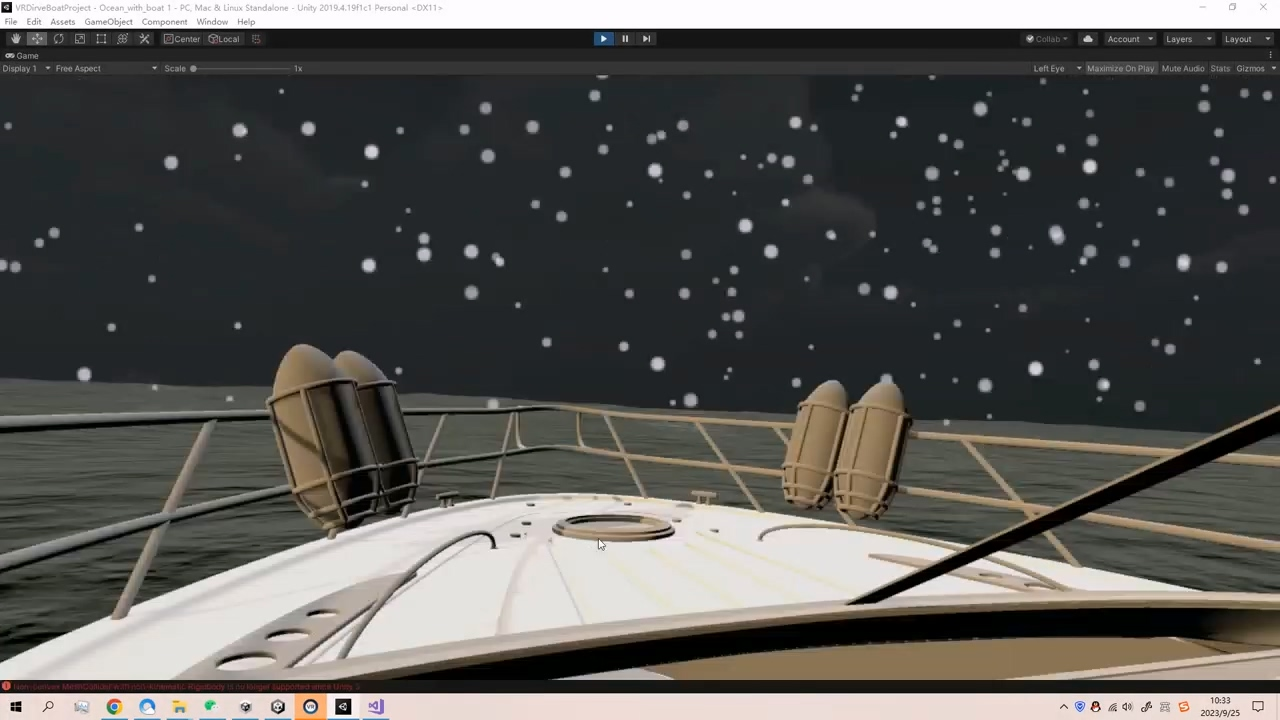
\includegraphics[width=\linewidth]{picture/First-person perspective Hail-IP}
				\captionsetup{font=scriptsize}
				\caption{First-person Hail}
				\label{fig: First-person perspective Hail-IP}	
			\end{subfigure}
			\begin{subfigure}{0.3\textwidth}
				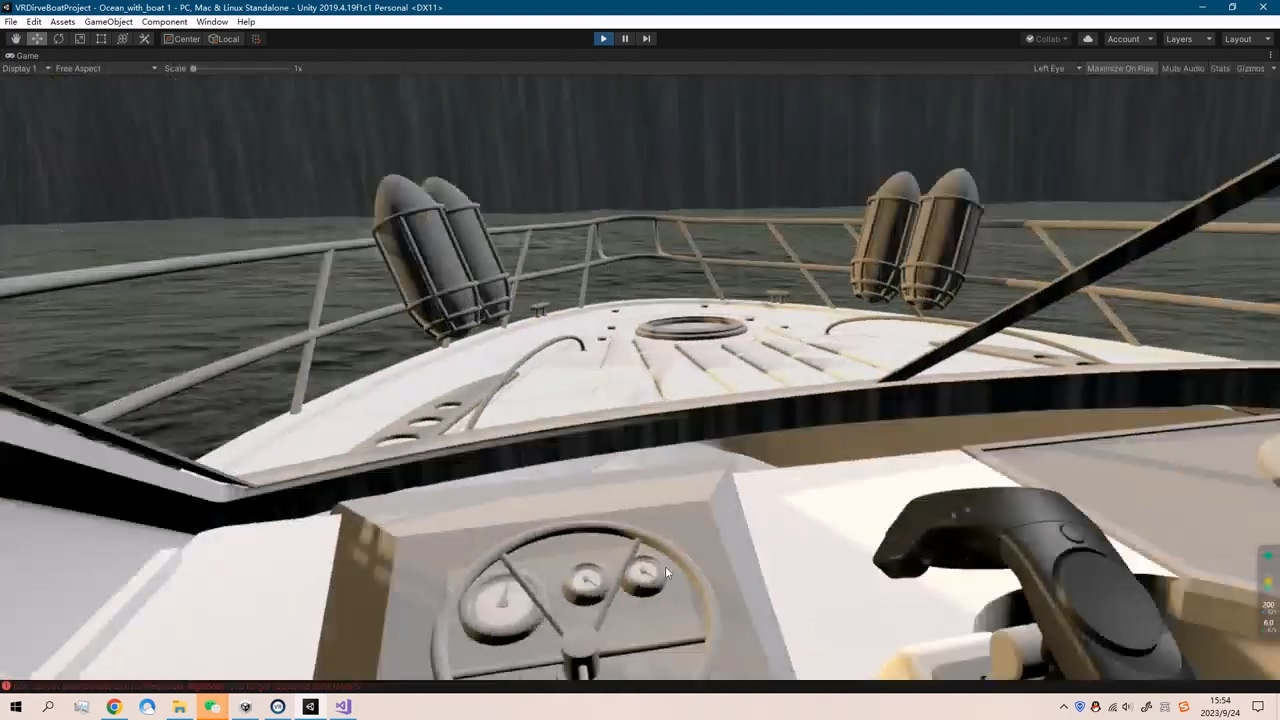
\includegraphics[width=\linewidth]{picture/First-person perspective rain-IP}
				\captionsetup{font=scriptsize}
				\caption{First-person Rain}
				\label{fig: First-person perspective rain-IP}	
			\end{subfigure}
			\begin{subfigure}{0.3\textwidth}
				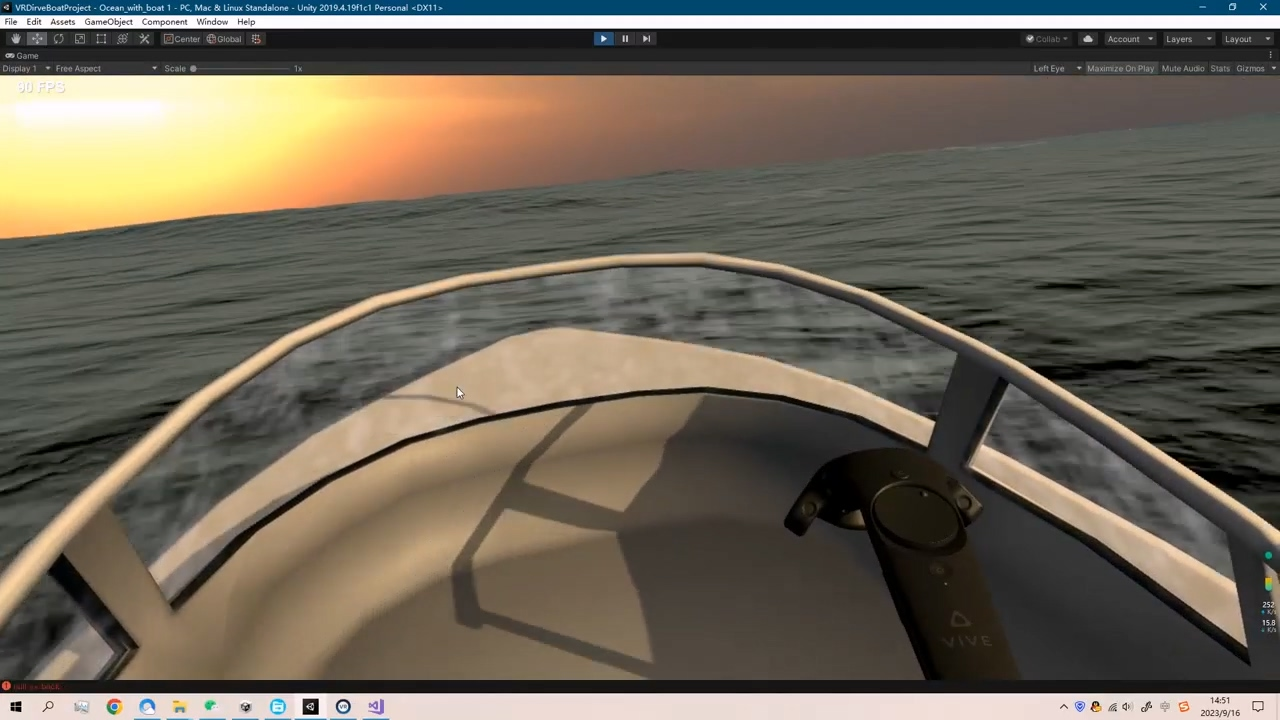
\includegraphics[width=\linewidth]{picture/First-person perspective-IP}
				\captionsetup{font=scriptsize}
				\caption{First-person Speedboat}
				\label{fig: First-person perspective-IP}	
			\end{subfigure}\\
			\begin{subfigure}{0.3\textwidth}
				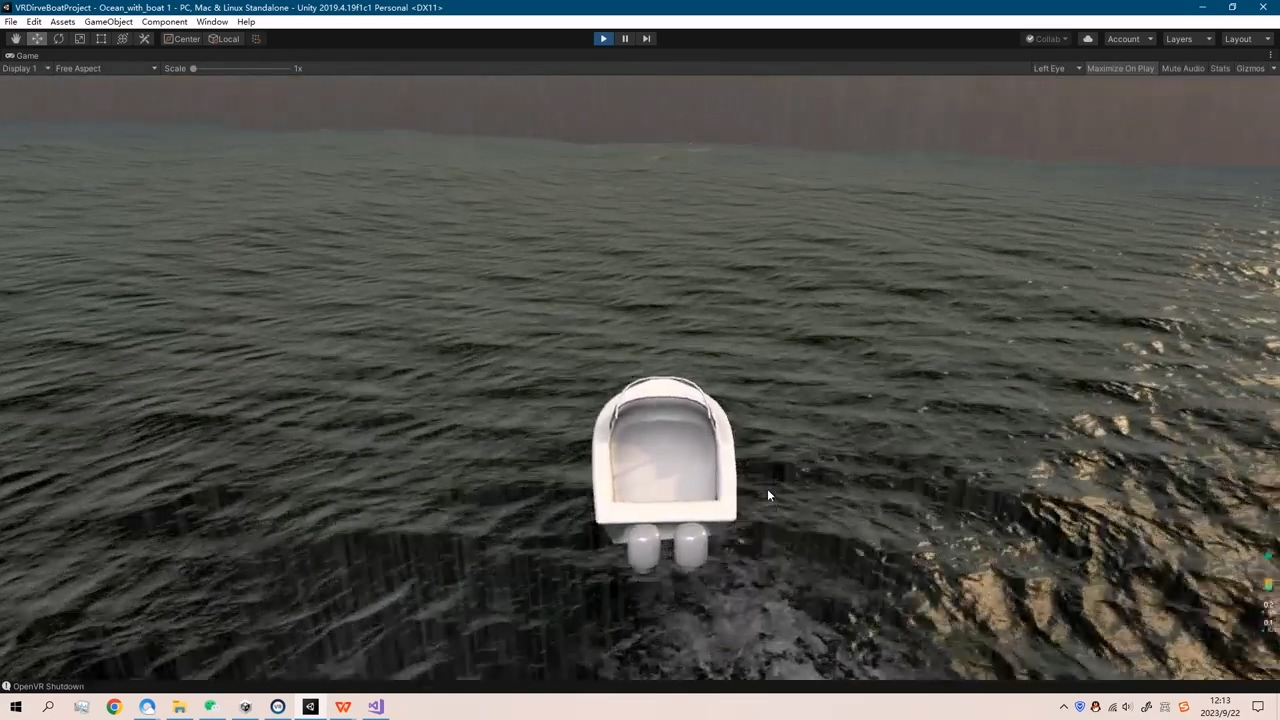
\includegraphics[width=\linewidth]{picture/Third-person perspective rain-IP}
				\captionsetup{font=scriptsize}
				\caption{Third-person Speedboat}
				\label{fig: Third-person perspective rain-IP}	
			\end{subfigure}
			\begin{subfigure}{0.3\textwidth}
				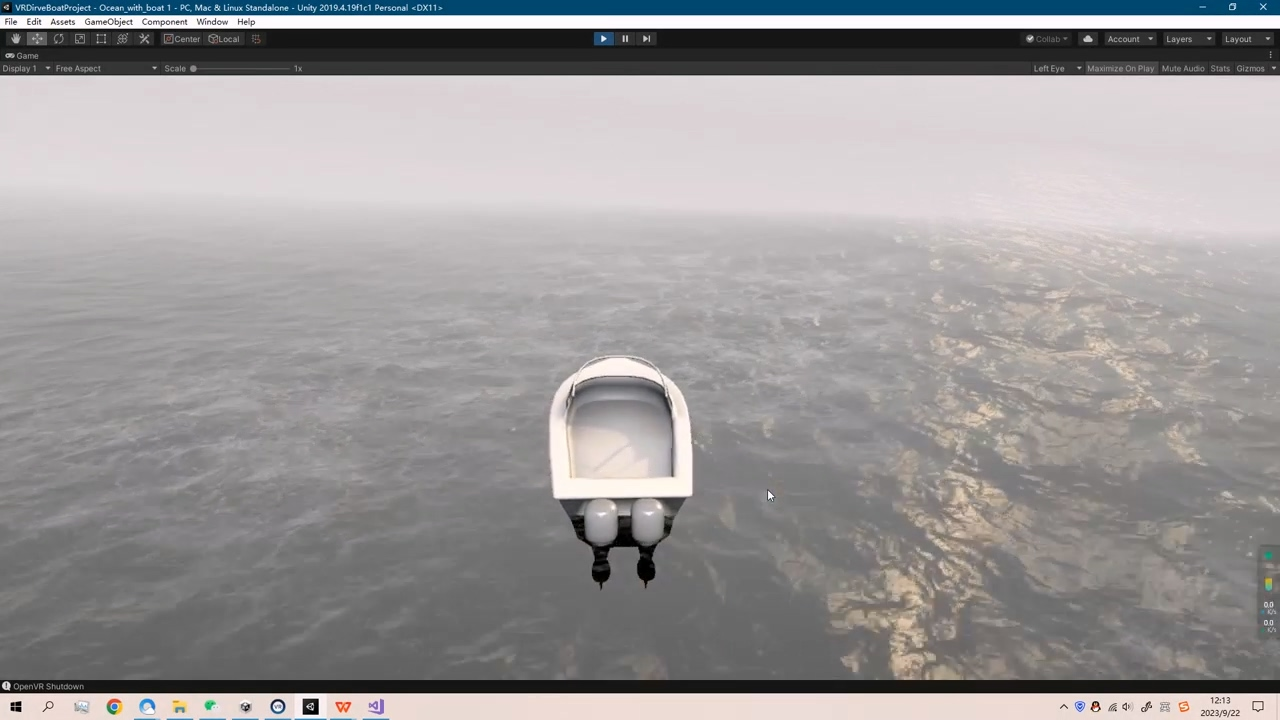
\includegraphics[width=\linewidth]{picture/Third-person perspective-IP}
				\captionsetup{font=scriptsize}
				\caption{Foggy Speedboat}
				\label{fig: Third-person perspective-IP}	
			\end{subfigure}
			\begin{subfigure}{0.3\textwidth}
				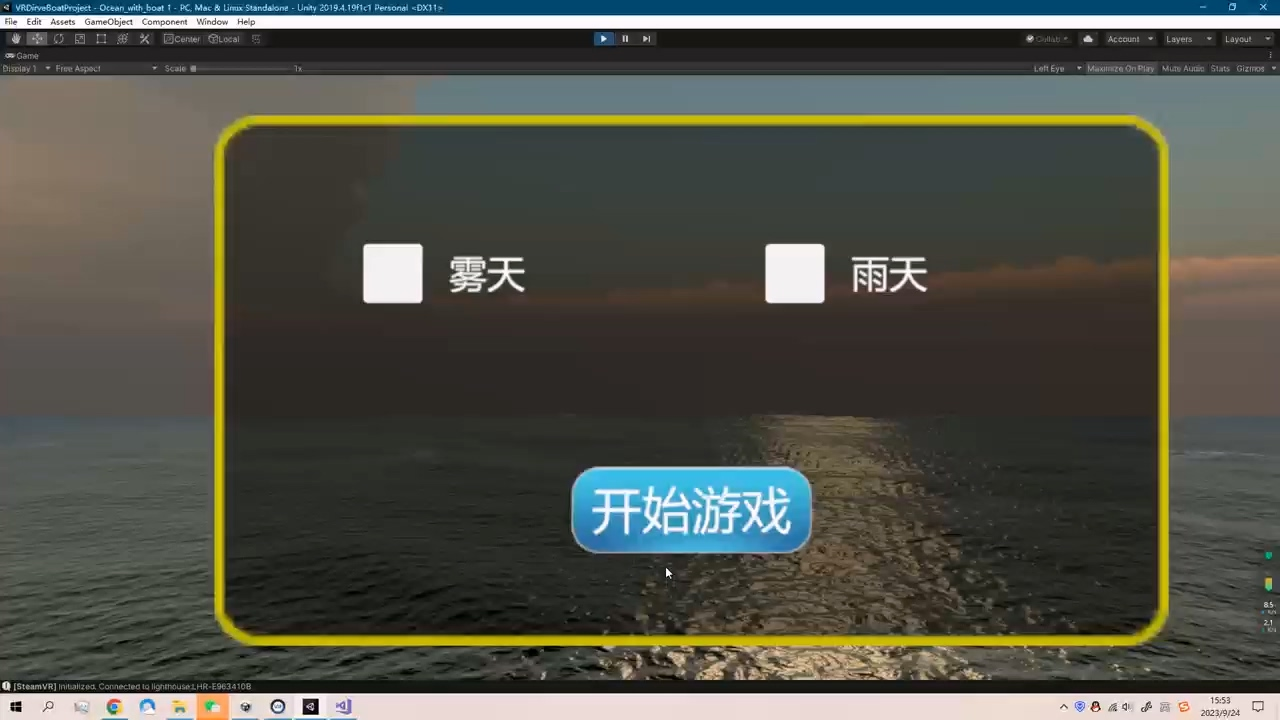
\includegraphics[width=\linewidth]{picture/Main menu-IP}
				\captionsetup{font=scriptsize}
				\caption{Main menu}
				\label{fig: Main menu-IP}	
			\end{subfigure}
			
			\captionsetup{font=scriptsize}
			\caption{
				\label{fig: Scene}						
			}
		\end{figure}
	
		\subsection{视角开发进度}
		
		玩家通过手柄摇杆按钮可以控制船只前进和后退,以及转向行驶,如 Fig. \ref{fig: First-person perspective rain-IP} 所示。
		
		玩家开船可以选择不同的船只视角,如 Fig. \ref{fig: Third-person perspective another hail-IP} 和 Fig .\ref{fig: First-person perspective Hail-IP} 所示。
		
		\subsection{船只模型}
		
		目前选择了两种船只模型,见 Fig. \ref{fig: Third-person perspective another-IP} 和 Fig. \ref{fig: Third-person perspective-IP}
		
		\subsection{未来开发计划}
		
		基于构建 VR 沉浸式体验装置的需求,计划通过添加游戏控制器震动反馈作为对气缸控制的前期调研,以期解决目前气缸无序运动的问题。同时计划在 VR 游戏中构建更合理的海洋水系统,以期构建更多样化的天气场景。		
		

	%	\section{Analysis}
	
	%	In this section you will need to show your experimental results. Use tables and
	%	graphs when it is possible. Table~\ref{tbl:bins} is an example.
	
	%	\begin{table}[ht]
		%		\begin{center}
			%			\caption{Every table needs a caption.}
			%			\label{tbl:bins} % spaces are big no-no withing labels
			%			\begin{tabular}{|ccc|} 
				%				\hline
				%				\multicolumn{1}{|c}{$x$ (m)} & \multicolumn{1}{c|}{$V$ (V)} & \multicolumn{1}{c|}{$V$ (V)} \\
				%				\hline
				%				0.0044151 &   0.0030871 &   0.0030871\\
				%				0.0021633 &   0.0021343 &   0.0030871\\
				%				0.0003600 &   0.0018642 &   0.0030871\\
				%				0.0023831 &   0.0013287 &   0.0030871\\
				%				\hline
				%			\end{tabular}
			%		\end{center}
		%	\end{table}
	%	
	%	Analysis of equation~\ref{eq:aperp} shows ...
	%	
	%	Note: this section can be integrated with the previous one as long as you
	%	address the issue. Here explain how you determine uncertainties for different
	%	measured values. Suppose that in the experiment you make a series of
	%	measurements of a resistance of the wire $R$ for different applied voltages
	%	$V$, then you calculate the temperature from the resistance using a known
	%	equation and make a plot  temperature vs. voltage squared. Again suppose that
	%	this dependence is expected to be linear~\cite{Cyr}, and the proportionality coefficient
	%	is extracted from the graph. Then what you need to explain is that for the
	%	resistance and the voltage the uncertainties are instrumental (since each
	%	measurements in done only once), and they are $\dots$. Then give an equation
	%	for calculating the uncertainty of the temperature from the resistance
	%	uncertainty. Finally explain how the uncertainty of the slop of the graph was
	%	found (computer fitting, graphical method, \emph{etc}.)
	%	
	%	If in the process of data analysis you found any noticeable systematic
	%	error(s), you have to explain them in this section of the report.
	%	
	%	It is also recommended to plot the data graphically to efficiently illustrate
	%	any points of discussion. For example, it is easy to conclude that the
	%	experiment and theory match each other rather well if you look at
	%	Fig.~\ref{fig:samplesetup} and Fig.~\ref{fig:exp_plots}.
	%	
	%	\begin{figure}[ht] 
		%		\centering
		%		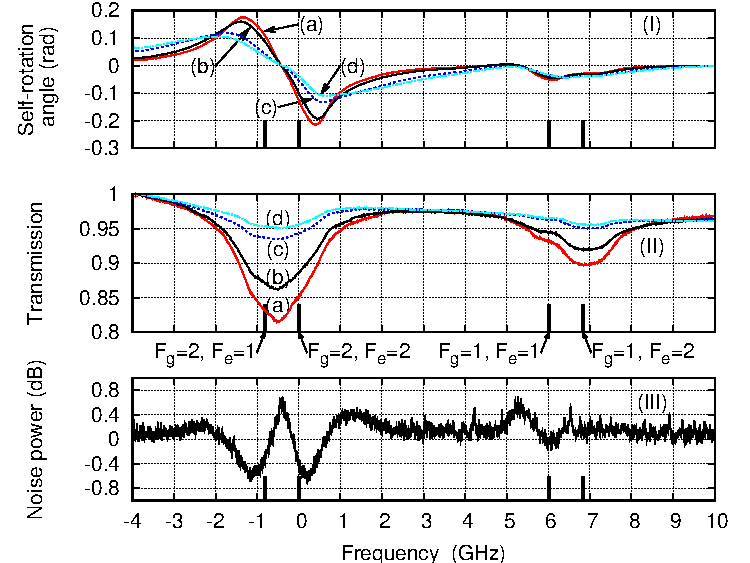
\includegraphics[width=0.5\columnwidth]{sr_squeezing_vs_detuning}
		%		
		%		% some figures do not need to be too wide
		%		\caption{
			%			\label{fig:exp_plots}  
			%			Every plot must have axes labeled.
			%		}
		%	\end{figure}
	
	
	%	\section{Conclusions}
	%	Here you briefly summarize your findings.
	
	%++++++++++++++++++++++++++++++++++++++++
	% References section will be created automatically 
	% with inclusion of "thebibliography" environment
	% as it shown below. See text starting with line
	% \begin{thebibliography}{99}
		% Note: with this approach it is YOUR responsibility to put them in order
		% of appearance.
		
%		\renewcommand{\refname}{References}
		
		
		%	\begin{thebibliography}{00}
			
			%		\bibitem{b1}\label{cite:b1}
			%		W. Wang, C. Wei, W. Yang and J. Liu, "GLADNet: Low-Light Enhancement Network with Global Awareness," 2018 13th IEEE International Conference on Automatic Face \& Gesture Recognition (FG 2018), Xi'an, China, 2018, pp. 751-755, DOI: 10.1109/FG.2018.00118.
			
			%		\bibitem{b2}\label{cite:b2}
			%		A.\ Mahajan, K.\ Somaraj and M. Sameer, "Adopting Artificial Intelligence Powered ConvNet To Detect Epileptic Seizures," 2020 IEEE-EMBS Conference on Biomedical Engineering and Sciences (IECBES), Langkawi Island, Malaysia, 2021, pp. 427-432, DOI: 10.1109/IECBES48179.2021.9398832.
			
			%		\bibitem{Cyr}
			%		N.\ Cyr, M.\ T$\hat{e}$tu, and M.\ Breton,
			% "All-optical microwave frequency standard: a proposal,"
			%		IEEE Trans.\ Instrum.\ Meas.\ \textbf{42}, 640 (1993).
			
			
			
			%	\end{thebibliography}
		
%		\bibliographystyle{unsrt}
%		\bibliography{reference}
		
		
	\end{document}
